\documentclass[a4paper,11pt]{article}
\usepackage[utf8]{inputenc}    % Codificación de caracteres
\usepackage[spanish]{babel}    % Soporte para español
\usepackage{amsmath}           % Paquete matemático
\usepackage{amssymb}           % Símbolos adicionales
\usepackage{hyperref}          % Enlaces en el documento
\usepackage{geometry}          % Configuración de márgenes
\usepackage{fancyhdr}          % Cabeceras y pies de página
\usepackage{enumitem}          % Control sobre listas
\usepackage{tikz}              % Para diagramas y gráficos
\usepackage{listings}          % Código fuente
\usepackage{graphicx}          % Insertar imágenes
\usepackage{tcolorbox}         % Cuadros gricess.
\usepackage{longtable}
% Configuración de los márgenes
\geometry{top=2.5cm, bottom=2.5cm, left=2.5cm, right=2.5cm}

% Configuración de cabeceras y pies de página
\pagestyle{fancy}
\fancyhf{}
\fancyhead[L]{CCNA Notes}  % Cabecera izquierda
\fancyhead[R]{\thepage}    % Cabecera derecha con número de página

% Definir un entorno para definiciones
\newtheorem{definition}{Definición}

% Título y autor
\title{Apuntes del Curso CCNA}
\author{Alejandro}
\date{\today}

\begin{document}

% Título y tabla de contenidos
\maketitle
\tableofcontents
\newpage

\section{Host Roles}
\begin{itemize}
    \item Hosts are devices assigned an IP address for communication.
    \item Clients (a type of host) use software like web browsers to request and display information from servers.
\end{itemize}

\subsection{Peer-to-Peer}
It is possible for one computer to be used for both roles at the same time.

\begin{tcolorbox}[colframe=gray!80, colback=gray!20, coltitle=black, title=Peer-to-Peer]
    The advantages of peer-to-peer networking:
    \begin{itemize}
        \item Easy to set up.
        \item Less complex.
        \item Lower cost because network devices and dedicated servers may not be required.
        \item Can be used for simple tasks such as transferring files and sharing printers.
    \end{itemize}
    The disadvantages of peer-to-peer networking:
    \begin{itemize}
        \item No centralized administration.
        \item Not as secure.
        \item Not scalable.
        \item All devices may act as both clients and servers, which can slow their performance.
    \end{itemize}
\end{tcolorbox}

\subsection{End Divices}
\begin{itemize}
    \item End devices are the network devices people typically use.\\
    \item Each end device  has a unique address for identification.\\
    \item Communication between end devices involves using their address to route messages.\\
    \item An end device act as either the source of the destination for the date transmitted over the network.\\
\end{itemize}

\subsection{Intermediary Devices}
\begin{itemize}
    \item Role: They connect and devices to the network and can link multiples networks to create an internet-work.\\
    \item Function: They ensure date flows  smoothly across the network by determining the message path using the destination address and network interconnections.\\
\end{itemize}
% Ejemplo del cuadro con información en grises y blancos
\begin{tcolorbox}[colframe=gray!80, colback=gray!20, coltitle=black, title= Peer-to-Peer]
     Intermediary network devices perform some or all of these functions:
    \begin{itemize}
        \item Regenerate and retransmit communication signals.\\
        \item Maintain information about what pathways exist through the network and internet-work.\\
        \item  Notify other devices of errors and communication failures.\\
        \item Direct date along alternate pathways when there is a link failure.\\
        \item Classify and direct messages according to priorities.\\        \item Permit or deny the flow of date, based on security settings.\\
    \end{itemize}
    Note: Not shown is a legacy Ethernet hub. An Ethernet hub is also known as a multi-port repeater. Repeaters regenerate and retransmit communication signals. Notice that all intermediary devices perform the function of a repeater.\\
\end{tcolorbox}

\begin{figure}[h!]
    \centering
    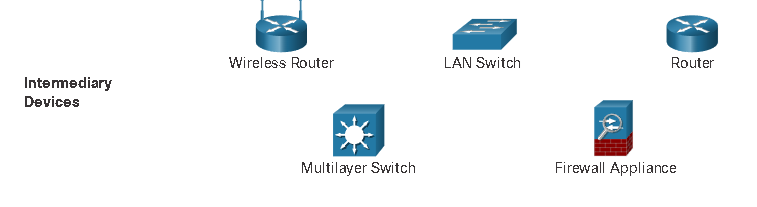
\includegraphics[width=\textwidth]{1.png}
    \caption{Intermediary Devices}
    \label{fig:cap1}
\end{figure}

\subsection{Network Media}
All about how data travels across the network.\\

% Ejemplo del cuadro con información en grises y blancos
\begin{tcolorbox}[colframe=gray!80, colback=gray!20, coltitle=black, title= Network Media]
     The four main criteria for choosing network media are these:\\
    \begin{itemize}
        \item What is the maximum distance that the media can successfully carry a signal?\\
        \item What is the environment in which the media will be installed?\\
        \item What is the amount of date and at what speed must it be transmitted?\\
        \item What is the cost of the media and installation?\\
    \end{itemize}
    
\end{tcolorbox}
\subsubsection{Cooper}
\begin{itemize}
\item UTP Cables: Made of 8 copper wires twisted into 4 pairs, typically ending in RJ-45 connectors.\\
\item Coble Types:\\
\begin{enumerate}
\item Straight-through cables: Connects corresponding pins on both ends.\\
\item Crossover cables: connects transmitting pins on one end to receiving ping on the other.\\
\end{enumerate}
\item Auto-MDIX featue: Some devices(like Cisco's) auto-detect incorrect cable usage and adjust accordingly, Though this isn't always the case.\\
\item Wrong cable Issues: Using an incorrect cable type(e.g., crossover cable) with auto-MDIX disabled results in the interface being down.\\
\item Auto-MDIX: Enabling auto-MDIX allows the switch to automatically adjust and use the correct pins, resolving the issue and bringing the interface up.\\
\end{itemize}

\lstset{language=bash}
\begin{lstlisting}
Switch# configure terminal
Switch(config)# interface fastethernet 0/1
Switch(config-if)# mdix auto   % Enable auto-MDIX
Switch(config-if)# no mdix auto   % Disable auto-MDIX
\end{lstlisting}

\subsubsection{Fiber-optic}
\begin{itemize}
    \item Fiber optics basics: Uses light pulses(digital signals) instead of electrics pulses.\\
    \item Optical Core: Glass tubes reflect light signals for transmission. Smaller cores allow signals to travels farther.\\
    \item Multi-mode Vs. Single Mode:\\
    \begin{enumerate}
        \item Multi-mode: Bigger core(50um, 62.5um), shorter distances. Used LED light source.\\
        \item Single Mode: Smaller core(8um, 9um), longer distances, Uses laser light source.\\
    \end{enumerate}
    \item Wavelengths: Different colors (wavelengths) of light travel without interference, important for data transmission.\\
\end{itemize}

\subsubsection{Wireless}
\begin{itemize}
    \item Wireless Communication Types: Covers applications like ratio, TV, radar, cellular, GPS, WIFI, Bluetooth, and RFID.\\
    \item Wife Bands:\\
    \begin{enumerate}
        \item 2.4GHz: longer range, slower speeds.\\
        \item 5GHZ: Shorter range, faster speeds, less interference but should not be confused with cellular 5G.\\
    \end{enumerate}
\end{itemize}

\subsection{Network Representation and Topologies}

\begin{itemize}
    \item Network Topology Diagrams: Visual representation of how devices connect, essential for understanding and planning networks.\\
    \item Physical Topology Diagrams: Show the physical location of devices and cables.\\
    \item Logical Topology Diagrams: Show how devices, ports, and addressing schemes are connected.\\
    \item  Key terms:\\
    \begin{enumerate}
        \item Network Interface Card(NIC): Connects end devices to the network.\\
        \item Physical Port: Outlet for media connections on devices.\\
        \item Interface: Port on networking devices, especially routers, that connect networks.\\
    \end{enumerate}
\end{itemize}

\begin{figure}[h!]
    \centering
    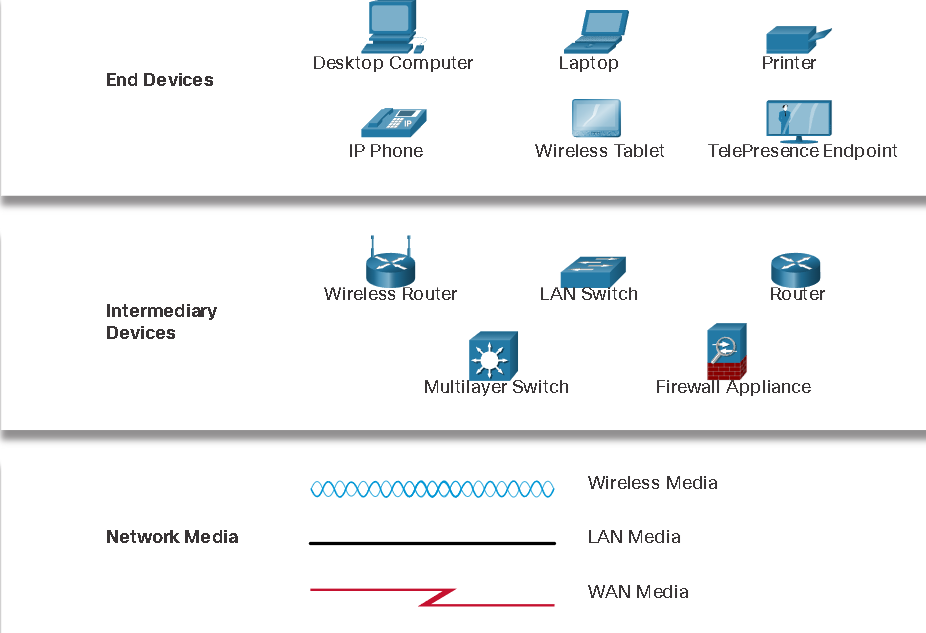
\includegraphics[width=\textwidth]{2.png}
    \caption{Intermediary Devices}
    \label{fig:cap1}
\end{figure}

\subsection{Common types of Networks}
\begin{itemize}
    \item Home Networks: Share resources like printers and files among a few devices.\\
    \item SOHO networks: Enable remote work and business operations.\\
    \item Business Networks: Support email, messaging, and data storage.\\
    \item Network Types:\\
    \begin{enumerate}
        \item Small Home Network: Connect a few devices and provide internet access.\\
        \item SOHO Networks: connect remote offices to corporate networks.\\
        \item: Mediam To Large Networks: Used by corporations, schools, covering multiple locations.\\
        \item World Wide Networks: The internet, connecting millions globally administration agencies like IETF, ICANN, and IAB.\\
    \end{enumerate}
    \item infrastructure Types:\\
    \begin{enumerate}
        \item LAN(Local Area Network): Small geographic area, like a home or small business(buildings, campus)\\
        \item WAN(Wide Area Network): Larger geographic areas, often managed by telecoms providers.\\
    \end{enumerate}
    \item Intranet: Private network for an organization's members or employees, typically connecting LANs and WANs.\\
    \item Extranet: Provides secure access to external users(e.g., suppliers, contractors) needing access to the organization's data.\\
\end{itemize}

\subsection{Internet connections}
\begin{itemize}
    \item Home/Small Office Connections: Options like broadband cable, DSL, cellular, satellite, and dial-up.\\
    \item Corporate connections: Require higher bandwidth and reliability, with options like business DSL, leased lines, metro Ethernet, and satellite.\\
    \item Converged Networks: Modern networks now integrate date, voice and video services over a single infrastructure, unlike traditional separate networks.\\
\end{itemize}

\subsection{Reliable Networks}
\begin{itemize}
    \item Reliability: Ensuring consistent and dependable network performance.\\
    \item Fault Tolerance: Redundancy and quick recovery mechanism to minimize the impact of failures.\\
    \item Scalability: ability to expand and support more users and applications without performance drops.\\
    \item Quality of Service(QoS): Prioritizing time- sensitive traffic to manage network congestion and ensure smooth data, voice, and video delivery.\\
    \item Network Security: Protecting infrastructure and information through confidentiality, integrity, and availability measures.\\
\end{itemize}

\subsection{Network Trends}
\begin{itemize}
    \item Bring Your Own Device(BYOD): Allow the use of the personal devices like laptops and smartphones for business of educational purposes, enabling flexibility and access from anywhere.\\
    \item Online Collaboration: Tools like Cisco WebEx facilitate teamwork and interaction among users, enhancing productivity and competitiveness.\\
    \item Video communications: Essential for communication and collaboration, video conferencing connects people globally and is crucial for effective interaction.\\
    \item Cloud Computing: enables date storage and access over the internet.\\
    \begin{enumerate}
        \item Public Clouds: Accessible to the general population, often free of pay-per-use.\\
        \item Private Clouds: Dedicated to a single organization with strict security.\\
        \item Hybrid Clouds:Combination of public and private clouds.\\
        \item Community Clouds: Shared among organizations with similar needs, like healthcare with special compliance requirements.\\
    \end{enumerate}
    \item Smart Home Technology: Integration of everyday appliances with networked devices for automation and remote control. Examples included smart ovens and calendars.\\
    \item Power line Networking: Uses existing electrical wiring to connect devices to the LAN, useful where wireless signals don't reach.\\
    \item Wireless Broadband:  Connectivity options where cable and DSL aren't available, utilizing WISPs and home wireless broadband solutions.\\
\end{itemize}

\subsection{Network Security}
\begin{itemize}
    \item Types of Threats:\\
    \begin{enumerate}
        \item External: Viruses, spyware, zero-day attacks. denial of service, data interception, and identity theft.\\
        \item Internal: Breaches due to last/stolen devices, employee misuse, and malicious insiders.\\
    \end{enumerate}
    \item Security Solutions:\\
    \begin{enumerate}
        \item Home Networks: Basic security like antivirus, anti-spyware, and firewall filtering.\\
        \item Corporate Networks: Advanced systems including dedicated firewalls, ACLs, IPS, and VPNs.\\
    \end{enumerate}
    \item Key Concepts:\\
    \begin{enumerate}
        \item Layered Security: Multiple solutions for enhanced protection.\\
        \item Adaptability: Solutions must evolve with network trends.\\
    \end{enumerate}
\end{itemize}

\newpage
\section{Cisco IOS Access}
\subsection{Operating Systems}
\begin{itemize}
    \item 1. Operating System (OS) Components:\\
    \begin{enumerate}
        \item Kernel: Manages communication Between hardware and Software; allocated resources to meet software requirements.\\
        \item Shell: User interface that interacts with the OS, allowing user to request tasks via:\\
        \begin{itemize}
            \item CLI(Command-Line Interface): Text-based, requires command knowledge, lightweight, stable.\\
            \item GUI(Graphical User Interface): Icon/menu, user-friendly, requires less command knowledge, but more resource-intensive and can be less stable.\\
        \end{itemize}
    \end{enumerate}
    \item Comparions: CLI vs GUI\\
    \begin{enumerate}
        \item CLI: Direct interaction with system via text commands, low resource use, stable, commonly used for network devices.\\
        \item GUI: Easy to use, but heavier on resources and potentially less stable; typically used by general users.\\
    \end{enumerate}
    \item Network Device OS:\\
    \begin{itemize}
        \item Cisco IOS: The main OS  used on Cisco routers and switches, with different versions for different devices(e.g., ISO XE, IOS XR, NX-OS).\\
        \item Home Router OS (Firmware): Usually configured via a web-based GUI.\\
    \end{itemize}
    \item Why use CLI  for network devices?: More stable, uses fewer resources, and provides access to advanced features that GUIs may not offer.\\
\end{itemize}
\subsection{Purpose of an OS}
\begin{itemize}
    \item Purppose of an OS in Networking:\\
    \begin{itemize}
        \item Similarities with PC OS: Allows user interaction via GUI (mouse, text input, output on a monitor).\\
        \item CLI:\\
        \begin{itemize}
            \item Uses keyboard for commands.\\
            \item Output text on monitor.\\
        \end{itemize}
    \item Cisco IOS Version: Different devices run different version of Cisco IOS based on device type and required features: IOS can be upgraded for more capabilities.\\
    \end{itemize}
    \item Access Method for Configuring Network Devices:\\
    \begin{itemize}
        \item Console Port(Out-of-band Access):\\
        \begin{itemize}
            \item A physical port used for initial configuration or device maintenance.\\
            \item Accessible without networking service configured.
            \item Requires a console cable and terminal emulation software.\\
        \end{itemize}
        \item SSH (In-band Access):\\
        \begin{itemize}
            \item Secure, encrypted connection via a virtual interface.\\
            \item Requires networking services(active interface with an IP address).\\
            \item Recommended for secure remote CLI access.\\
        \end{itemize}
        \item Telnet(in-band Access):\\
        \begin{itemize}
            \item Unsecured, sends in plain-text.\\
            \item Should only be used in lab environments.\\
            \item Not recommended for real-world used -- SSH is preferred.\\
        \end{itemize}
        \item AUX Port(Out-of-band Access):\\
        \begin{itemize}
            \item Legacy port used for remote access over telephone connection via a modem.\\
            \item Like console ports, it doesn't require networking services.\\
        \end{itemize}
        \item Switch Configuration:\\
        \begin{itemize}
            \item Switches forward(send) traffic by default, but it's recommended to configured and secure all switches even though they operate by default.\\
        \end{itemize}
        \item Best Practice:\\
        \begin{itemize}
            \item Use SSH instead of Telnet for secure remote access.\\
            \item Console of AUX ports are useful when no networking service are available.\\
        \end{itemize}
    \end{itemize}
\end{itemize}

\subsection{IOS Navigation}
\begin{itemize}
    \item User EXEC Mode: This is a basic "View-only" mode with limited commands, mainly for monitoring. The prompt ends with \ $>$.\\
    \item Privileged EXEC Mode: This mode allows full access to all commands, including configuration and management. It's accessed from User EXEC mode using the  enable command, and its prompt ends with \#.\\
    \item Configuration Mode: This is used for device-wide configuration changes. It's  accessed from Privileged EXEC mode with the configure terminal command. The prompt changes to (config)\#.\\
    \item Sub configuration Modes:\\
    \begin{enumerate}
        \item Line configuration Mode: Configures access methods like console, SSH, and Telnet. The prompt is (config-line)\#\\
        \item Interface Configuration Mode: Configures switch ports or routes interfaces. The prompt is (config-if)\#\\
    \end{enumerate}
\end{itemize}

% Ejemplo del cuadro con información en grises y blancos
\begin{tcolorbox}[colframe=gray!80, colback=gray!20, coltitle=black, title= EXEC mode]
    
    \begin{itemize}
        \item Use Enable to move to Privileged EXEC mode.\\
        \item Use exit to return to the previous mode, or CTRL + Z to return directly to Privileged EXEC mode.\\
        \item You can switch directly between sub configuration mode using specific commands, e.g., interface for interface configuration.\\
    \end{itemize}
\end{tcolorbox}

\subsection{Basic Device Configuration}
The first step in configure any network device is to give it a unique hostname to easily identify it withing the network. The default name on a cisco switch is "Switch," but leaving all switches with the same name can lead to confusion, especially when then remotely via SSH.\\

% Ejemplo del cuadro con información en grises y blancos
\begin{tcolorbox}[colframe=gray!80, colback=gray!20, coltitle=black, title= Hostname Guidelines]
     To avoid confusion and ensure easy identification, follow these naming conventions:\\
    \begin{itemize}
        \item Start with a letter(mnemonic: Alphabet starts your identity)\\
        \item No spaces (mnemonic: One name, no gaps).\\
        \item End with a letter or digit  (Mnemonic: Close it strong).\\
        \item Only use letters, digits, and dashes (mnemonic: keep it simple).\\
        \item Less than 64 characters (mnemonic: Shorter is easier to remember).\\
    \end{itemize}
\end{tcolorbox}


% Ejemplo del cuadro con información en grises y blancos
\begin{tcolorbox}[colframe=gray!80, colback=gray!20, coltitle=black, title= Example]
    Examples in a network with multiples floors, switches can be named based on their location and purpose. For instance, Sw-Floor-1 for the switch on the first floor.\\
    \begin{itemize}
        \item  Swith\# configure terminal.\\
        \item  Switch(config)\# hostname Sw-Floor-1.\\
        \item  Sw-Floor-1(config)\#.\\
    \end{itemize}
     To reset the hostname back to the default, use no hostname.\\
\end{tcolorbox}

\subsection{Password Configuration}
Security is essential, and weak password ar a common issue. Use strong passwords to secure network devices. should:\\
\begin{itemize}
    \item Be at least 8 characters long.\\
    \item Include uppercase, lowercase, numbers, and symbols.\\
    \item Avoid common words.\\
    \item Be unique for each device.\\
\end{itemize}
% Ejemplo del cuadro con información en grises y blancos
\begin{tcolorbox}[colframe=gray!80, colback=gray!20, coltitle=black, title= Example]
     User EXEC Mode Password(Console Access):\\
    \begin{itemize}
        \item Sw-Floor-1(config)\# configure terminal\\
        \item Sw-Floor-1(config)\#  line console 0\\
        \item Sw-Floor-1(config)\# password xxxxxxxx\\
        \item Sw-Floor-1(config)\# login\\
    \end{itemize}
     To reset the hostname back to the default, use no hostname.
     To secure privileged EXEC mode, use the enable secret command:\\
     \begin{itemize}
         \item Sw-Floor-1(config)\# enable secret class\\
     \end{itemize}
\end{tcolorbox}

% Ejemplo del cuadro con información en grises y blancos
\begin{tcolorbox}[colframe=gray!80, colback=gray!20, coltitle=black, title= Securing Remote Access (VTY Lines)]
     To secure VTY lines (for SSH/Telnet), use the following commands:\\
    \begin{itemize}
        \item Sw-Floor-1(config)\# configure terminal\\
        \item Sw-Floor-1(config)\# line vty 0 15\\
        \item Sw-Floor-1(config)\# password xxxxxxx\\
        \item Sw-Floor-1(config)\# login\\
    \end{itemize}
     
\end{tcolorbox}

% Ejemplo del cuadro con información en grises y blancos
\begin{tcolorbox}[colframe=gray!80, colback=gray!20, coltitle=black, title= Recap]
     
    \begin{itemize}
        \item Hostname: Make sure it  is descriptive and unique for easy identification.\\
        \item Passwords: Ensure they are strong and varied to prevent unauthorized access.\\
        \item Documentation: Always update network documentation with names and password for future reference.\\
    \end{itemize}
\end{tcolorbox}

% Ejemplo del cuadro con información en grises y blancos
\begin{tcolorbox}[colframe=blue!80, colback=blue!20, coltitle=black, title= Scenario:  Helping a customer configure a hostname and password for a cisco switch]
     
    \begin{itemize}
        \item You: Hello, thanks for contacting cisco support! My name is Alejandro, how may I assist you today?\\
        \item Customer: Hi Alejandro, I need help configuring my switch. I'm setting up a network and I need to change the hostname and set a password for security.\\
        \item You: I can definitely help with that! Let's go through the process step by step. I'll walk you through configuring the hostname first, and then we'll set up a password to secure your switch. Are you at the command line of your switch right now?\\
        \item You: Great! First, let's make sure we're in the correct mode. Could you please type enable and press Enter? This will put us into privileged EXEC mode.\\
        \item Customer: Okay, I've done that.\\
        \item You: Perfect! Now we need to enter global configuration mode. Type configure terminal and press Enter. You should see the prompt change to something like Switch(config)\#.\\
        \item Customer: Yes, I see that now.\\
        \item You: Excellent! now let's give your switch a unique hostname. This will help identify it easily on the network. You can type the following command: hostname Myswitch-1 and press enter. You can replace my switch-1 with any name you prefer.\\
        \item Customer: Okay, I've don that and I see the name changed in the prompt.\\
        \item You: Perfect! your switch now has a new hostname. Now let's secure your switch by setting a password for privileged access. Are you ready for the next steps?\\
    \end{itemize}
\end{tcolorbox}
% Ejemplo del cuadro con información en grises y blancos
\begin{tcolorbox}[colframe=blue!80, colback=blue!20, coltitle=black, title= Scenario:Handling Potential Issues with Patience]
     If the customer encounter an issue, such as typing an incorrect command, guide them calmly without making them feel rushed.\\
    \begin{itemize}
        \item Customer: wait, I think I typed something wrong, It's not working.\\
        \item You: No problem, let's fix that together. Could you read the command back to me so I can check it?\\
        \item You: Ah, I see the issue. Let's try again. The command should be hostname followed by a space and then your desired name. Let me know when you're ready.\\
        \item Customer: Okay, that worked!\\
        \item You: Great job! let's move on to securing the switch with a password. This will help prevent unauthorized access.\\
    \end{itemize}
\end{tcolorbox}
% Ejemplo del cuadro con información en grises y blancos
\begin{tcolorbox}[colframe=blue!80, colback=blue!20, coltitle=black, title= Scenario:Guiding Through Password Configuration]
      Use clear, jargon-free language, and reassure the customer tht they're on the right track.\\
    \begin{itemize}
        \item  You: We'll now set the password for privileged EXEC mode. To do this, you'll type enable secret followed by the password you want. For example, you can type enable secret strongpassword. Make sure it's something secure, and avoid common words.\\
        \item Customer: Done! It accepted the password.\\
        \item You: Awesome! Now, Just to confirm, we'll save these changes. Go ahead and type end to exit configuration mode, then type write memory or copy running-config startup-config to save the changes.\\
        \item Customer: All saved!\\
    \end{itemize}
\end{tcolorbox}
% Ejemplo del cuadro con información en grises y blancos
\begin{tcolorbox}[colframe=blue!80, colback=blue!20, coltitle=black, title= Scenario:Closing with Reassurance and follow-up]
      Before ending the call, make sure the customer is confident with the changes and ask if they need nay further  help.\\
    \begin{itemize}
        \item  You: You've done a great job configuring your switch today! It now has a unique hostname and a secure password in place. Is there anything else I can assist you with?\\
        \item Customer: No, that's all I needed. Thanks so much for your help!\\
        \item You: You're very welcome! if you need help in the future, don't hesitate to reach out. Have a great day and good luck with your network setup!\\
    \end{itemize}
\end{tcolorbox}

\subsection{The Command Structure}
\begin{itemize}
    \item Command Syntax:\\
    \begin{enumerate}
        \item Cisco IOS commands have a specific structure involving keywords and arguments.\\
        \item Keywords are predefined parameters(e.g, ip protocols) set by the system.\\
        \item Arguments are values provided by the user, such as an IP address(e.g., "192.168.10.5").\\
        \item Commands are entered in the appropriate mode, and after typing the complete command, pressing enter submits it.\\
    \end{enumerate}
    \item Command Syntax indicators:\\
    \begin{enumerate}
        \item Boldface text: Represents commands or keywords that must be entered exactly as shown.\\
        \item Italic text: Represent arguments where the user supplies values.\\
        \item Square brackets []: Indicate optional elements in a command.\\
        \item Braces {}: Indicate required elements.\\
        \item Braces with vertical lines [x{y$\|z$}]: Represent a required chose within an optional element.\\
    \end{enumerate}
    \item Examples of Commands Used:\\
    \begin{enumerate}
        \item Simple command: ping ip-address (e.g., ping 10.10.10.5) send a ping request to an IP address.\\
        \item More complex command: Switch(config-if)\# switchport port-security aging \{static $\|$ time time $ \|$ type \{ absolute $\|$ inactivity\}\} requires a choice between options.\\
    \end{enumerate}
    \item Command Documentation:\\
    \begin{enumerate}
        \item Each Cisco command is documented, detailing its syntax and possible argument.\\
        \item For example, the command description  allows the user to add a description to an interface, like identifying its purpose ("description connects to the main headquarter office switch").\\
    \end{enumerate}
\end{itemize}
% Ejemplo del cuadro con información en grises y blancos
\begin{tcolorbox}[colframe=blue!80, colback=blue!20, coltitle=black, title= Scenario: General Idea:]
Understanding the structure of IOS command is essential for network administrator. Each command has a specific format with keywords and user-defined arguments. The command syntax is clearly defined using text formats like bold and italics to distinguish between what must be entered as-is and what the user needs to provide. Knowing how to ready and use this syntax is key to configuring network devices correctly.\\  
\end{tcolorbox}
\subsection{Hot Keys and Shortcuts}
Cisco IOS provides built-in help feature and shortcuts to make command-line navigation and device configuration more efficient. Using context-sensitive help and command syntax check prevents errors by offering guidance on commands and their correct structure. Additionally, hot keys simplify command editing, and tools like the "\--More\--" prompt help manage long outputs. Overall, understanding these tools makes working in the CLI faster and more intuitive.\\
\begin{enumerate}
    \item Key Points: 
    \begin{itemize}
        \item Use the "?" to quickly identify which commands or arguments are available in the current mode.\\
        \item It helps you discover valid commands based on what you've typed so far, ensuring correct used.\\ 
    \end{itemize}
    \item Command Syntax Check:\\
    \begin{itemize}
        \item IOS checks if commands are valid as they are typed. If the command is correct, executes; if incorrect, an error message explains the issues.\\
    \end{itemize}
    \item Hot Keys and Shortcuts:\\
    \begin{itemize}
        \item The CLI offers various shortcuts for command editing, improving speed and ease of use.\\
        \item Example: Typing conf instead of configure works because "conf" uniquely identifies the command, but "con"  doesn't because it could be ambiguous.\\
        \item keystrokes like Tab out-complete commands, while others like CTRL + a or CTRL + E allow quick cursor movement to the beginning or end of a line.\\
    \end{itemize}
    \item More Output Handling:\\
    \begin{itemize}
        \item If the command output exceeds the display, the "--More--" prompt appears. Press Enter to display the next line, Space for the next screen, or another key to exit.\\ 
    \end{itemize}
    \item Exiting Modes of Operations:\\
    \begin{itemize}
        \item CTRL + C: Exits configuration mode and returns to the privileged EXEC mode aborts an operation.\\
        \item CTRL + Z: ends configuration mode and return to privileged EXEC.\\
        \item CTRL + Shift + 6: Interrupts processes like DNS lookups, traceroutes, or ping.\\
    \end{itemize}
\end{enumerate}

% Ejemplo del cuadro con información en grises y blancos
\begin{tcolorbox}[colframe=blue!80, colback=blue!20, coltitle=black, title= Scenario: set up the clock]
\begin{lstlisting}[language=bash, caption={Clock Configuration on a Cisco Device}]
Switch> enable
Switch# show clock
*00:30:05.261 UTC Mon Mar 1 1993

Switch# clock set 15:30:00 Dec 03 2024
Switch# show clock
15:30:00 UTC Tue Dec 3 2024
Switch#
\end{lstlisting}
\end{tcolorbox}

% Ejemplo del cuadro con información en grises y blancos
\begin{tcolorbox}[colframe=blue!80, colback=blue!20, coltitle=black, title= Scenario: set up the clock]
\begin{itemize}
    \item agent: Alright! Let us set up the clock on your Cisco device. I will guide you step by step-it is straightforward, and I will explain each step as we go. Are you ready to get started?\\
    \item Customer: "Yes, I'm ready!"\\
    \item Agent: "Great! First, make sure you're logged into your device through the console. Once you're in, you'll see a prompt, like switch> or Router>. Let me know when you see that."\\
    \item Customer: "Yest, I'm at switch>."\\
    \item Agent: "Perfect. Now, to set the clock, we need to access a more advanced mode called "Privileged EXEC mode." to do this, type enable and press Enter. The prompt will change to Switch \#. Did that work?"\\
    \item Customer: "Yes, I'm at Switch \# now."\\
    \item Agent: "Excellent! Next, we'll use the command clock set. This command lets us input the current time and date. The at is hh:mm:ss DAY  MONTH YEAR. Let's try setting the time to 2:30 pm on December 3, 2024. Type this exactly: clock set 14:30:00 Dec 3 2024, then press Enter."\\
    \item Customer: "Done, It didn't  give me any errors."\\
    \item Agent: "Fantastic! To confirm it's set correctly, type show clock and press enter. This will desplay the current clock settings. What does it say?"\\
    \item Customer: "It says 14:30:00 UTC Tue Dec 3 2024."\\
    \item Agent: "Perfect! The clock is now set up correctly. Keep i mind that setting the correct time is important, especially for troubleshooting and login events. Do you have any other question about this process?"\\
    \item Customer: "No, this was very helpful. Thank you!"\\
    \item Agent: "You're welcome! Feel free to reach out if you need further assistance. Have a great day!"\\
    \end{itemize}
\end{tcolorbox}

\subsection{Basic Device Configuration}
Configuring Cisco devices involves settings unique hostname, strong passwords, encryption, and legal banner to ensure secure and manageable networks. Proper naming conventions, strong password policies, and clear documentation streamline administration and bolster(help) security.\\
\begin{itemize}
    \item Configure Example:\\
    \begin{enumerate}
        \item Enter global configuration mode: configure terminal.\\
        \item Assign a hostname: hostname [name].\\
        \item Restor to default: no hostname.\\
    \end{enumerate}
    \item Password best Practices:\\
    \begin{enumerate}
        \item Use password > 8 characters with a mix of upper/lowercase letters, numbers, and symbols.\\
        \item Avoid common words or repeating passwords.\\
        \item Utilize password generators for complexity.\\
        \item Use service password-encryption to apply basic encryption to stored passwords.\\
        \item Validate encryption with show running-config.\\
    \end{enumerate}
    \item Banner configuration:\\
    \begin{enumerate}
        \item command: banner motd \# [message] \#\\
        \item The \# is a delimiter, and any unique symbols can replace it, provided it's not part of the massage.\\
    \end{enumerate}
\end{itemize}

% Ejemplo del cuadro con información en grises y blancos
\begin{tcolorbox}[colframe=blue!80, colback=blue!20, coltitle=black, title= Scenario: Basic Configuration]
\begin{lstlisting}[language=bash, caption={Configuration on a Cisco Device}]
Switch> enable
Switch# clock set 15:30:00 Dec 03 2024
Switch# show clock
15:30:00 UTC Tue Dec 3 2024
Switch# 
Switch# configure terminal
Switch(config)# hostname Sw-Floor-1
Sw-Floor-1(config)# banner motd #no authorized access only# 
Sw-Floor-1(config)# line console 0
Sw-Floor-1(config)# password [password]
Sw-Floor-1(config)# login    
\end{lstlisting}
Sw-Floor-1(config)# login   -->this ensures the device asks for the password before granting access.\\
\end{tcolorbox}

% Ejemplo del cuadro con información en grises y blancos
\begin{tcolorbox}[colframe=blue!80, colback=blue!20, coltitle=black, title= Scenario: Securing User EXEC mode (Console Access)]
 To secure privileged EXEC access, use the enable secret password global config command, as shown in the example.\\
\begin{lstlisting}[language=bash, caption={Configuration on a Cisco Device}]
Sw-Floor-1# configure terminal
Sw-Floor-1(config)# enable secret [password]
Sw-Floor-1(config)# exit
Sw-Floor-1#
\end{lstlisting}
\end{tcolorbox}



% Ejemplo del cuadro con información en grises y blancos
\begin{tcolorbox}[colframe=blue!80, colback=blue!20, coltitle=black, title= Scenario: Securing Using Telnet SSH]
  Virtual terminal(VTY) lines enable remote access using Telnet of SSH to the device. To secure VTY lines, enter line VTY mode using the line vty0 15 global config command.\\
\begin{lstlisting}[language=bash, caption={Configuration on a Cisco Device}]
Sw-Floor-1# configure terminal
Sw-Floor-1(config)# line vty 0 15
Sw-Floor-1(config)# password [password]
Sw-Floor-1(config)# login
Sw-Floor-1(config)# end
Sw-Floor-1#
\end{lstlisting}
\end{tcolorbox}

% Ejemplo del cuadro con información en grises y blancos
\begin{tcolorbox}[colframe=blue!80, colback=blue!20, coltitle=black, title= Scenario: Securing Using Telnet SSH]
  Virtual terminal(VTY) lines enable remote access using Telnet of SSH to the device. To secure VTY lines, enter line VTY mode using the line vty0 15 global config command.\\
\begin{lstlisting}[language=bash, caption={Configuration on a Cisco Device}]
Sw-Floor-1# configure terminal
Sw-Floor-1(config)# line vty 0 15
Sw-Floor-1(config)# password [password]
Sw-Floor-1(config)# login
Sw-Floor-1(config)# end
Sw-Floor-1#
\end{lstlisting}
\end{tcolorbox}

% Ejemplo del cuadro con información en grises y blancos
\begin{tcolorbox}[colframe=blue!80, colback=blue!20, coltitle=black, title= Scenario: Encrypt Passwords]
  To encrypt all plaintext passwords, use the service-encrypton global config command.\\
\begin{lstlisting}[language=bash, caption={Configuration on a Cisco Device}]
Sw-Floor-1# configure terminal
Sw-Floor-1(config)# service password-encryption
Sw-Floor-1(config)# 
\end{lstlisting}
Use the show running-config command to verify that password are now encrypted.\\
\end{tcolorbox}

\subsection{Save Configurations}
\begin{enumerate}
    \item Types of configuration:\\
    \begin{itemize}
        \item startup-config:\\
          \begin{itemize}
            \item Stored in NVRAM (non-volatile memory).\\
            \item Contains the saved configuration that the device uses when starting up or rebooting.\\
            \item Retains data even when the device is powered off.\\
         \end{itemize}
        \item Runing-config:\\
         \begin{itemize}
            \item Stored in RAM(volatile memory).\\
            \item Reflects the current configuration and takes effect intermediately upon modification.\\
            \item Lost when the device is restarted is restarted of powered off unless saved to the startup-config.\\
          \end{itemize}
         \item viewing configuration\\
          \begin{itemize}
             \item Use show running-config to view the current (active) configuration in RAM.\\
             \item Use show startup-config to view the saved configuration in NVRAM.\\
          \end{itemize}
         \item Saving configuration:\\
           \begin{itemize}
             \item Used the command copy cunning-config startup-config to save the current active configuration to NVRAM, ensuring it persists after a reboot.\\
           \end{itemize}
          \item Restoring configuration:\\
            \begin{itemize}
              \item If changes to the running-config are not desirable:\\
               \begin{itemize}
                   \item Removed individual changes manually.\\
                   \item Use the reload command to revert the startup-config.\\
                   \item During reload, you will prompted to save changes. Respond with no to discard the unsaved changes.\\
               \end{itemize}
               \item If  the startup-config contains unwanted setting:\\
               \begin{itemize}
                   \item use the erase startup-config to remove it, followed by a reload to reset the device to its default factory settings.\\
               \end{itemize}
            \end{itemize}
    \end{itemize}
    \item caution with the reload and erase commands:\\
    \begin{itemize}
        \item using reload causes temporay network downtime as the device restart.\\
        \item erase startup-config removes all saved configuration, requiring a fresh setup after reload.\\
    \end{itemize}
\end{enumerate}

% Ejemplo del cuadro con información en grises y blancos
\begin{tcolorbox}[colframe=blue!80, colback=blue!20, coltitle=black, title= Scenario: Copying the running configuration to the startup configuration]
Copying the running configuration to the startup configuration:
switch\# copy running-config startup-config
Success\\

Copying the running configuration to a new checkpoint named ckpt1:\\

switch\# copy running-config checkpoint ckpt1
Success\\

If we want to save this running config, we can copy it to the startup configuration:\\
\begin{lstlisting}[language=bash, caption={Configuration on a Cisco Device}]
R1#copy running-config startup-config
Destination filename [startup-config]? 
Building configuration...
[OK]
\end{lstlisting}

When we copy the running configuration to whatever destination, it will always overwrite the destination file. Let’s try that:\\
\begin{lstlisting}[language=bash, caption={Configuration on a Cisco}] R1#copy running-config my-config.cfg
Destination filename [my-config.cfg]? 
1072 bytes copied in 1.076 secs (996 bytes/sec)
\end{lstlisting}

The first time I save the running configuration as “my-config.cfg” the file does not exist. The second time I do this, it will overwrite the file:\\
\begin{lstlisting}[language=bash, caption={Configuration on a Cisco}]
R1#copy running-config my-config.cfg
Destination filename [my-config.cfg]? 
%Warning:There is a file already existing with this name 
Do you want to over write? [confirm]

1072 bytes copied in 0.648 secs (1654 bytes/sec)
\end{lstlisting}
\end{tcolorbox}

\begin{figure}[h!]
    \centering
    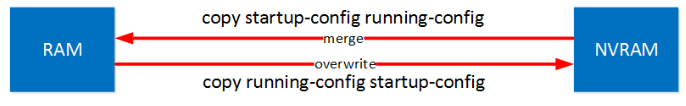
\includegraphics[width=\textwidth]{3.png}
    \caption{Intermediary Devices}
    \label{fig:cap1}
\end{figure}
 
\begin{lstlisting}[language=bash, caption=Switch Configuration]
Switch> enable
Switch#
Switch# clock set hh:mm:ss month day year
Switch# show clock
15:30:00 UTC Tue Dec 3 2024
Switch# show running-config
Switch# configure terminal
Switch(config)# hostname S1
S1(config)# line console 0
S1(config-line)# password letmein
S1(config-line)# login
S1(config-line)# line vty  0 15
S1(config-line)# password [password]
S1(config-line)# login
S1(config)# enable password c1$c0
S1(config)# enable secret itsasecret--> replace c1$c0
S1(config)# service password$-$encryption
S1(config)# banner motd "This is a secure system. Authorized Access Only!"
S1(config)# exit
S1# copy running-config startup-config
\end{lstlisting}

\subsection{IP ADDRESS}
To enable device communication on a network. Each device must have a valid IP address. IPV4 and IPV6 are the key protocols for addressing, and IPV6 is designed for the growing needs of the Internet. Network connections rely on specific physical interfaces and media types, and switches use virtual interfaces (SVIs) for remote management, emphasizing the importance of correctly configuring IP addresses and the network.\\

\begin{itemize}
    \item IPv4
    \begin{enumerate}
        \item Requires a subnet mask to identify the network and host portion of the address (e.g., 255.255.255.0).\\
        \item Default Gateway: The router's IP address used for accessing other networks or the internet (e.g., 192.168.1.1).\\
    \end{enumerate}
    \item IPv6
    \begin{enumerate}
        \item Uses a 128-bit structure represented in hexadecimal, separated by colons(e.g., 2001:0db8:85a3::8a2e:0370:7334)\\
        \item Case-insensitive and allows shorthand notation for compact repressentaion.\\
    \end{enumerate}
    \item Network Interfaces:
    \begin{enumerate}
        \item Device communicate via physical interfaces (e.g., Ethernet ports) that adhere to specific standards.\\
        \item Network Media Types: Twisted-pair copper, fiber optics, coaxial cable, or wireless technologies.\\
        \item Media selection depend on factors like signal distance, environment, data speed, and cost.\\
    \end{enumerate}
    \item Ethernet:
    \begin{enumerate}
        \item The most common LAN technology with ports found on end-user and networking devices.\\
    \end{enumerate}
    \item Switch Ports:
    \begin{enumerate}
        \item Layer 2 switches have physical ports for connecting devices but do not directly support IP addresses.\\
        \item Instead, they use Switch virtual intefaces (SVIs) (e.g., VLAN1) for remote management via IP.\\
    \end{enumerate}
    \item Key Concepts:
    \begin{enumerate}
        \item SVI: A virtual inteface in layer 2 switches for remote manamvent using IPv4 or IPv6. It doesn't impact the switch's primary layer 2 operations.\\
        \item Switch IP Usage: Switches don't need IPs for functionality but require them for remote management.\\
    \end{enumerate}
\end{itemize}

\subsection{Swtich Virtual Interface configuration}
To access the switch remotely, an IP address and a subnet mask must be configured on the SVI. To configure an SVI on a switch, use the interface vlan 1 global configuration command. Vlan 1 is not an actual physical interface but a virtual one. Next assign an IPv4 address using the ip address ip-address subnet-mask interface configuration command. Finally, enable the virtual interface using the no shutdown interface configuration command.\\
Note: Similar to a Windows hosts, switches configured with an IPv4 address will typically also need to have a default gateway assigned. This can be done using the ip default-gateway ip-address global configuration command. The ip-address parameter would be the IPv4 address of the local router on the network, as shown in the example.\\

\begin{lstlisting}[language=bash, caption=Switch Configuration]
Sw-Floor-1# configure terminal
Sw-Floor-1(config)# interface vlan 1
Sw-Floor-1(config-if)# ip address 192.168.1.20 255.255.255.0
Sw-Floor-1(config-if)# no shutdown
Sw-Floor-1(config-if)# exit
Sw-Floor-1(config)# ip default-gateway 192.168.1.1
\end{lstlisting}

\newpage
\section{The Rules}

\subsection{Message Formatting and Encapsulation}
Just like a letter must be formatted correctly for delivery, network messages must also follow specific format rules to be delivered successfully. \textbf{Encapsulation} refers to placing a message inside another format (like putting a letter in an envelope). For networks, protocols like \textbf{IPv6} encapsulate the message with addressing information (sender and receiver).\\

\subsection{Message Size}
In communication, messages are often broken into smaller, manageable parts. Similarly, \textbf{network messages} are broken into \textbf{frames}. These frames must follow specific size rules to be properly delivered and reassembled at the destination.\\

\subsection{Message Timing}
\begin{itemize}
    \item \textbf{Flow Control}: Manages the rate of data transmission to prevent overwhelming the receiver.\\
    \item \textbf{Response Timeout}: Defines how long a device will wait for a response before deciding how to proceed (e.g., retrying or moving on).\\
    \item \textbf{Access Method}: Manages when devices can send messages, preventing simultaneous transmissions (which could result in collisions).\\
\end{itemize}

\subsection{Message Delivery Options}
\begin{itemize}
    \item \textbf{Unicast}: Sending a message to a single device.\\
    \item \textbf{Multicast}: Sending a message to multiple devices.\\
    \item \textbf{Broadcast}: Sending a message to all devices on a network.\\
\end{itemize}
\subsection{Protocols}
Network protocols are a set of rules that enable communication between devices over a network. These protocols define common formats and rules for exchanging messages. They are implemented in software, hardware, or both and vary depending on the function, format, and communication requirements.\\

\subsection{Types of Network Protocols:}
\begin{longtable}{|l|p{10cm}|}
\hline
\textbf{Type of Protocol} & \textbf{Description} \\
\hline
\endfirsthead

\hline
\textbf{Type of Protocol} & \textbf{Description} \\
\hline
\endhead

\hline
\textbf{Network Communications Protocols} & These protocols allow devices to communicate across networks, such as IP, TCP, and HTTP. \\
\hline
\textbf{Network Security Protocols} & Used for data protection through encryption, authentication, and integrity. Examples include SSH, SSL, and TLS. \\
\hline
\textbf{Routing Protocols} & Enable routers to exchange routing information and determine the best path. Examples include OSPF and BGP. \\
\hline
\textbf{Service Discovery Protocols} & Automatically detect devices and services. Examples include DHCP (for IP address allocation) and DNS (for name-to-IP address translation). \\
\hline

\end{longtable}

\subsection{Network Protocols Functions}
\begin{itemize}
    \item Addressing: Identifies the sender and reveiver(e.g., Ethernet, IPv4, IPv6).\\
    \item Reliability: Ensures message delivery, often through TCP.
    \item Flow control: Menages data transmission speed to ensure efficient communication(e.g., TCP).\\
    \item Sequencing: Labels data segments for correct reassembly in case of delays or loss (e.g., TCP).\\
    \item Error Detection: Detects corrupted date during transmission(e.g., Ethernet, IPv4, TCP).\\
    \item Application Interface: Manages communication between network applications(e.g., HTTP, HTTPS for web pages).\\
\end{itemize}


\subsection{Protocols Suites}
\begin{itemize}
    \item Protocols suites: A group of inter-related protocols necessary for network communication, designed to work together seamlessly.\\
    \item Protocols stack: Visualizes  how protocols within a suite interact, viewed as layers. Lower layers handle data movement while upper layer focus on message content.\\
\end{itemize}

\subsection{Examples of Protocols Suites}
\begin{itemize}
    \item Internet Protocols Suites(TCP/IP): The most common suite today, maintained by the IETF.\\
    \item Open Systems Interconnection (OSI): A layered model developed in 1977, largely replaced by TCP/IP.\\
    \item AppleTalk: A short-lived suite from Apple(1985-1995), replaced by TCP/IP.\\
    \item Novell NetWare: A suite from Novell(1983-1995).\\
\end{itemize}

\subsection{TCP/IP Protocols Suite}
\begin{itemize}
    \item Layers: Aplication, Transport, and Internet layers. Ethernet and WLAN are common Network Access Layer protocols.\\
    \item Characteristics:\\
    \begin{itemize}
        \item Open Standard: Freely available for used by any vendor.\\
        \item Standards-Based: Ensures interoperability between products from different manufactures.\\
    \end{itemize}
\end{itemize}

\begin{figure}[h!]
    \centering
    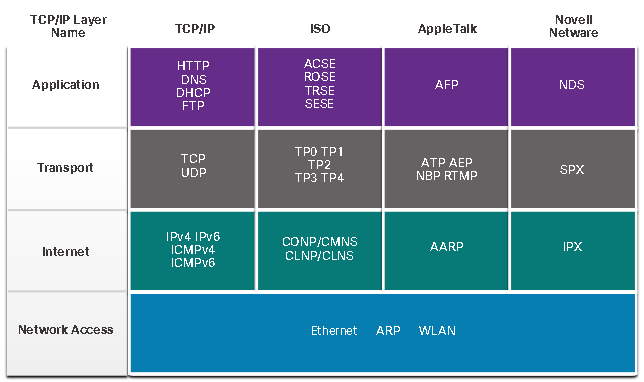
\includegraphics[width=0.75\textwidth]{4.png}
    \caption{TCP/IP}
    \label{fig:cap1}
\end{figure}

\subsubsection{TCP/IP}
Each protocol plays a unique role in ensuring efficient and secure network communication, from translating domain names to IP addresses (DNS) to securing file transfers (SFTP), and routing date (OSPF, BGP). Analogously, think of these protocols as different members of a team, each specializing in a specific task to keep the network running smoothly and securely.\\

\begin{enumerate}
    \item Application Layer: Represents data to the user, plaus encoding and dialog contorl. Here, you're using an app like emails or chat to send your message.\\
    \item Transport Layer: Supports communication between various devices across diverse networks. This layer makes sure your message arrives intact and in the right order, like a reliable delivery service.\\
    \item Internet Layer: Determines the best path through the network. Think of this as the GPS that finds the best route for your message to travel across the internet.\\
    \item Network Access: Control the hardware devices and media that make up the network. This is the actual road or path your message travels on, through cables or wireless signals.\\
\end{enumerate}

\begin{figure}[h!]
    \centering
    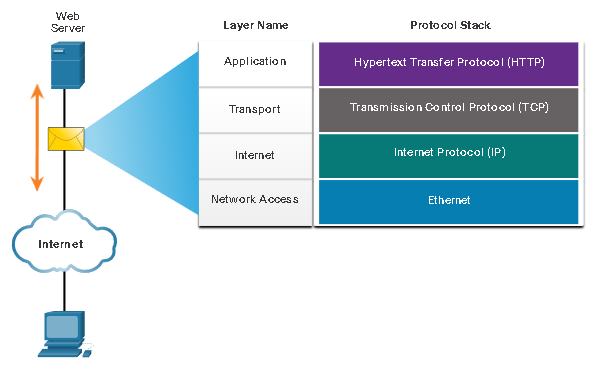
\includegraphics[width=0.75\textwidth]{5.png}
    \caption{TCP/IP}
    \label{fig:cap1}
\end{figure}

\subsection{Key Takeaways}
\begin{itemize}
    \item Interoperability: Protocols work togeether to provide comprehensive network communication.\\
    \item Layer Approach: Protocols are organized into layers, each with specific functions.\\
    \item  Adoption: TCP/IP has become the universal standard due to its open and standards-base nature.\\
\end{itemize}

\subsection{Reference Models OSI}
A layered model in networking helps manage complexity by breaking down tasks into layers, each with specific functions. This modular approach allows for standardization, compatibility, and easier troubleshooting, much like an assembly line in car manufacturing ensures each component fits and functions correctly. The OSI model, with its seven layers, serves as a foundational framework for understanding and implementing network protocols.\\

\begin{enumerate}
    \item Application Layer: Interface directly with user data. This is the content of your letter, where you write down your message. It directly interacts with you, the user.\\
    \item Presentation Layer: Preperes data for the application layer through translation, encryption, and compression.This is like translating your letter into a language your friend understands and making sure it's readable.\\
    \item Session Layer: Manages sessions between devices, ensuring data transfer completion, and using checkpoints for recovery. This layer is like the conversation between you and your friend about when you're going to send and receive letters.\\
    \item Transport Layer: Handles end-to-end communication, segmenting data and managing flow and error control. Imagine this layer  as a tracking system that ensures your letter is delivered correctly and safely.\\
    \item Network Layer: Transfers data between different networks, creating and routing packets. Protocols. This is the postal service that decides the best route to get your letter to your friend's city.\\
    \item Data Link Layer: Manages data transfer within the same network, creating and controlling frames. Think of this as a the envelop of your letter, ensuring it gets to the right place in the correct form.\\
    \item Physical Layer: Involves physical equipment and converts data to bits for transmission.  This is like the post office truck that physically carries your letter. It deals with the actual transmission of data.\\
\end{enumerate}

\begin{figure}[h!]
    \centering
    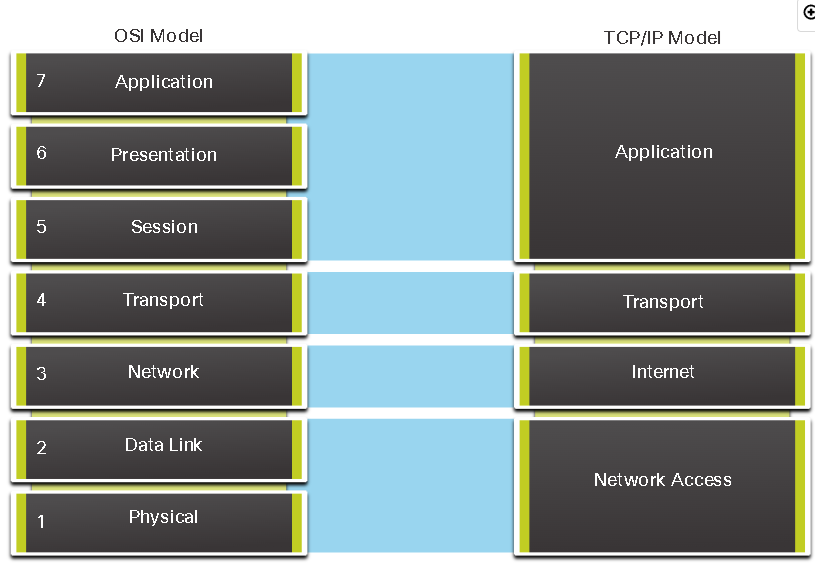
\includegraphics[width=0.75\textwidth]{6.png}
    \caption{TCP/IP OSI}
    \label{fig:cap1}
\end{figure}

\subsection{TCP/IP and OSI}\\
\begin{itemize}
    \item Application/Presentation/Session (OSI): The content and rules of communication.\\
    \item Transport: Reliable delivery and tracking.\\
    \item Network: finding the best path.\\
    \item Data link/Physical: Actual transmission over cables or airwaves.\\
\end{itemize}

\subsection{Data Encapsulation}
Networking involves breaking down larges data streams into smaller packets to ensure efficient and reliable transmission across the network. These packets are wrapped with protocols-specific information(encapsulation), Travel through various layers, and are then reassembled(sequencing) at the destination. This process is essential for maintaining speed and efficiency in data communication, much like sending multiple postcards instead of a single long letter ensures smoother and faster delivery.\\

\subsection{Segmenting Message}
\title{Encapsulation and Data Segmentation}\\
\begin{itemize}
    \item Encapsulation: When data moves across a network, it's wrapped in protocols information at each layer, much like nesting Russian dolls.\\
    \item Segmentation: Instead of sending a large message in one go (Which could clog(block, drag) the network), The message is divided into smaller, more manageable packets. Think of this llike sending a long letter as a series of postcards.\\
\end{itemize}

\title{Why Segmenting Matters}\\
\begin{itemize}
    \item Speed: Smaller packet travel faster and efficiently, enabling multiple conversations (like a busy post office handling many letters at once).\\
    \item Efficiency: If a packet fails to arrive, only that piece needs to be resent, not the entire message.\\
\end{itemize}

\title{Multiplexing and Sequencing}\\
\begin{itemize}
    \item Multiplexing and sequencing: Allows multiple data streams to share the same network path simultaneously.\\
    \item Sequencing: Ensures packets are reassembled in the correct order. Imagine sending a 100-page letter in 100 envelopes; each needs a number so they can be reordered correctly on arrival.\\
\end{itemize}

\title{Protocols data Units(PDUs)}\\
As data is encapsulated at each network layer, it tranformation into differents PDUs:\\
\begin{enumerate}
    \item Applicatio Layer: Data\\
    \item Transport Layer: Segment(Or Datagram if using UDP).\\
    \item Network Layer: Packet.\\
    \item Data link Layer: frame.\\
    \item Physical Layer: Bits.\\
\end{enumerate}

\begin{figure}[h!]
    \centering
    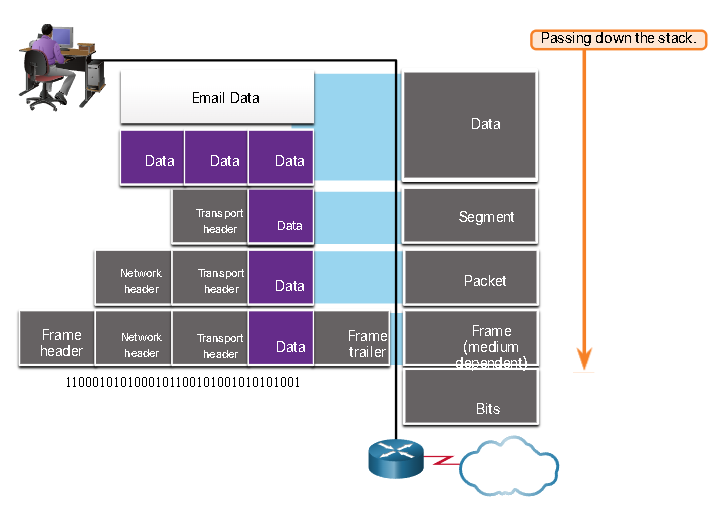
\includegraphics[width=0.75\textwidth]{7.png}
    \caption{PDUs}
    \label{fig:cap1}
\end{figure}

\subsection{Data Access}
Network addresses (IP and Mac) are assential for delivering messages across a network. IP address manage routing across different networks, while MAC addresses handle communication withing the same network. This layered addresses and zip codes to ensure mail reaches the right destination.\\

When devices are on a different netwoks, the data link facilitates communication by using MAC addresses and routes to direct frame. The IP packet is encapsulated in these  frames at each step, ensuring it is correctly delivered from the source to the final destination, much like passing a baton(stick) in arelay race. This layered approach ensures accurate and efficient date transmission across networks.\\

\begin{figure}[h!]
    \centering
    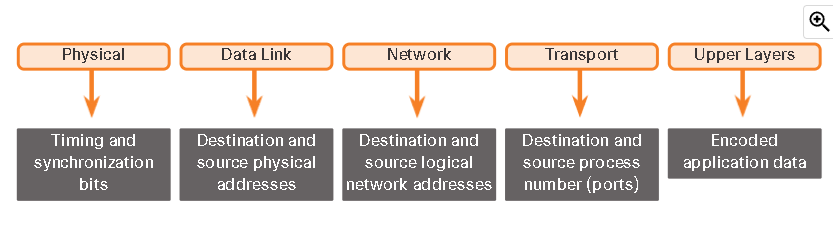
\includegraphics[width=0.75\textwidth]{8.png}
    \caption{PDUs}
    \label{fig:cap1}
\end{figure}

\title{Layer Responsabilities}\\
\begin{itemize}
    \item Network Layer: Uses IP addresses to deliver packets from the source to the final destination, whether on the same or a different network.\\
    \item Data Link: Uses Mac addresses to deliver frames within the same newtwork.\\
\end{itemize}

\title{IP Address structure}\\
\begin{itemize}
    \item Source IP Address: The IP address of the sending device.
    \item Destination IP Address: The IP of the receiving device.
    \item Parts of an IP Address:\\
        \begin{itemize}
            \item Network Portion: Identifies the network(left-most part)\\
            \item Host Portion Identifies the network(unique for each device.)\\
        \end{itemize}
\end{itemize}

\title{Same Network Communication}\\
\item Devices on the same network use their IP addresses and MAC addresses for communication.\\
\item Example: A plient PC (192.168.1.110) communicates with the FTP server (192.168.1.9) on the same network. They use MAC addresses fo direct data link frame delivery.\\

\title{Different Network Communication}\\
\begin{itemize}
    \item When devices are on different network, the network layer addresses (IP addresses) handle routing.\\
    \item Example: A client PC (192.168.1.110) communicates with web server (172.16.1.99) on a different network. The IP packet is routed accordingly.\\
\end{itemize}

\begin{figure}[h!]
    \centering
    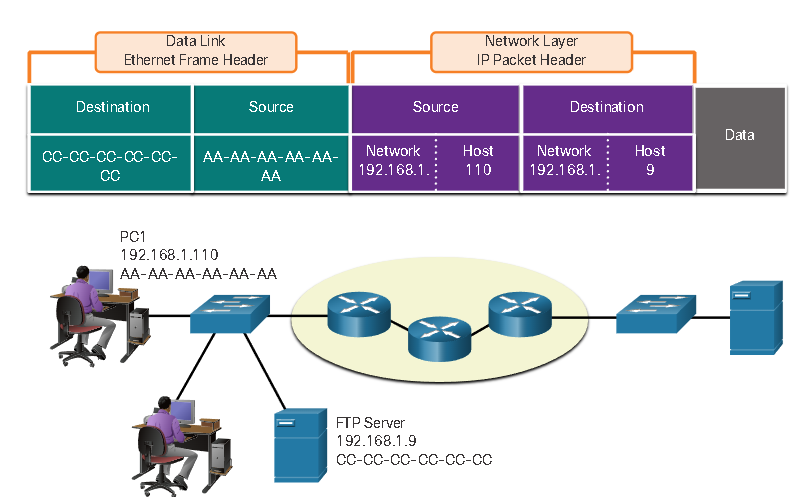
\includegraphics[width=0.75\textwidth]{9.png}
    \caption{PDUs}
    \label{fig:cap1}
\end{figure}

\title{Undestanding Data Link Layer Addresses}\\
when devices are on different networks, the data link layer Ethernet frames to help communicate. This involves the use of a router or default gateway since the destination device isn't directly reachable. Here's the simplified process:\\

\title{Communication Process}\\
\begin{itemize}
    \item Source MAC address: The MAC address o fthe sinding device (e.g., PC1).\\
    \item Destination MAC Address: The MAC address of the default gateway or router (e.g., R1) that is on the same network as the sending device.\\
\end{itemize}

\title{Example:}
\begin{itemize}
    \item PC1 has a source MAC address: AA-AA-AA-AA-AA-AA.\\
    \item The default gateway (R1) has a destination MAC address. 11-11-11-11-11-11.\\
\end{itemize}

The Ethernet frame with the IP packets is sent from PC1 to R1 then forwards the packet to its final destination, such a web server.\\

\title{Data Link Address and IP  Packets}\\
The data link handles the delivery of date frames within the same network. The IP packet travels encapsulated in these frames, with each frame containing.\\

\begin{itemize}
    \item Source Data Link Address: MAC address of the sending NIC.\\
    \item Destination Data Link Address: MAC address of the receiving NIC (either the next hop(setp, bound) router or the final destination).\\
\end{itemize}

\title{Host to Router, Router to Router to Server}\\
As the IP packet Travels:\\

\begin{figure}[h!]
    \centering
    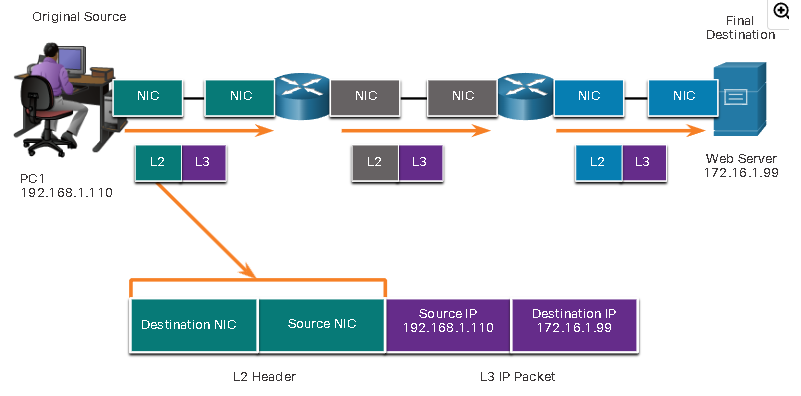
\includegraphics[width=0.75\textwidth]{10.png}
    \caption{Host to Router}
    \label{fig:cap1}
\end{figure}

\begin{figure}[h!]
    \centering
    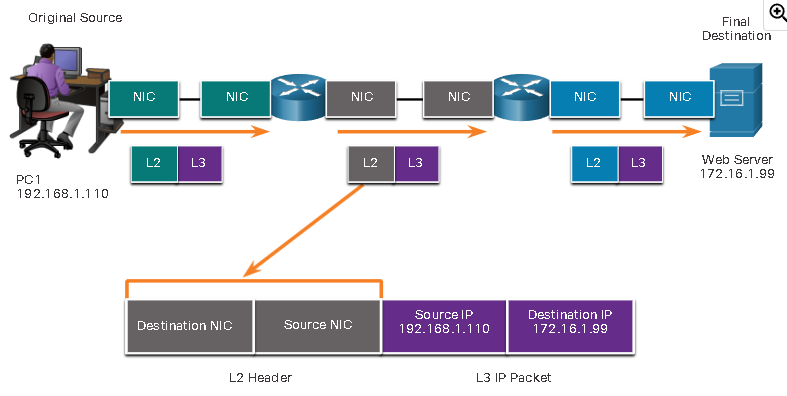
\includegraphics[width=0.75\textwidth]{11.png}
    \caption{Router to Router}
    \label{fig:cap1}
\end{figure}

\begin{figure}[h!]
    \centering
    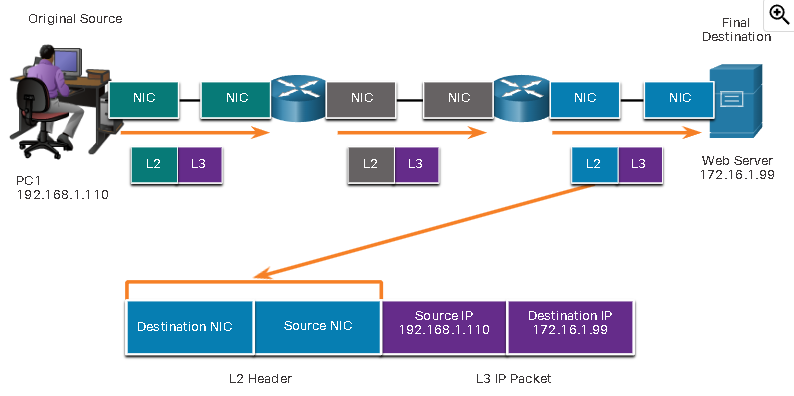
\includegraphics[width=0.75\textwidth]{12.png}
    \caption{Router to Server}
    \label{fig:cap1}
\end{figure}
\newpage
\begin{itemize}
    \item  From Host to Router, the router receives the updates the Layer 2 info.\\
    \item From Routers to Router, each router updates Layer 2 info for the next hop.\\
    \item Finally, Router to Server updates Layer 2 info until the packet reaches its destination.\\
\end{itemize}


\newpage
\section{Physical Layer}
\title{The Physical Connection}\\
To enable network communication, a physical connection must be established using either:\\
\begin{itemize}
    \item Wired Connections: Data is transmitted through Ethernet cables, typically connection devices like desktops or laptops to switches or routes.\\
    \item Wireless Connections: Data is transmitted using radio waves via wireless access points (APs) or wireless routes. Wirelss devices include laptops, tables, and smartphones.\\
\end{itemize}

\title{Access Point Components}\\
\begin{enumerate}
    \item Embedded wireless antennas.\\
    \item Ethernet switchports.\\
    \item Internet port.\\
\end{enumerate}

Devices use Newtwork Interface Cards (NICs) to connect to the network:\\
\begin{itemize}
    \item Ethernet NICs: for wired connections using Ethernet cables.\\
    \item WLAN NICs: For wireless connections using radio waves.\\
\end{itemize}

\title{The Physical Layer}\\
The physical layer of the OSI model is responsible for transmitting bits across network media by:\\
\begin{enumerate}
    \item Encoding Frames: Converts data link layer frames into electrical, optical, or radio wave signals.\\
    \item Transmitting Signals: Sends encoded bits over the network media.\\
    \item Receiving and Decoding: At the destination, the physical layer restores signals to their bit representation and forward the data to the data link layer.\\
\end{enumerate}

The process ensures reliable transmission of data through various media types(cables, radio waves, etc.), With each signal representing one bit at a time.\\

\subsection{Physical Layer Characteristics}
The physical layer in networking focuses on hardware, transmission media, and standards that enable communication at the lowest level of the OSI model.\\

\title{Standards Governing the Physical Layer}\\
The physical layer is governed by hardware and media standards developed by engineering organizations, such as:\\
\begin{itemize}
    \item Iso: International Organization for Standardization.\\
    \item TIA/EIA: Telecommunications Industry Association/Electronic Industries Association.\\
    \item IEEE: Institute of Electrical and Electronics Engineers.\\
    \item FCC (USA) and ETSI (Europe): National and regional telecommunications regulators.\\
\end{itemize}
These standards ensure compatibility and uniformity in physical components, signaling, and encoding globally.\\

\title{Functional Area Addressed by Physical Layer Standards}\\
\begin{enumerate}
    \item Physical Components\\
    \begin{itemize}
        \item Includes hardware devices, media, connectors, and cable materials.\\
        \item Examples: NICs, ports, interface, and connectors(e.g., on Cisco 1941 routes).\\
    \end{itemize}
    \item Encoding\\
    \begin{itemize}
        \item Converts data bits into a recognizable code for transmission.\\
        \item Encoding patterns provide predictability for both sender and receiver.\\
        \item Example: Manchester Encoding (used in 10 Mbps Ethernet) represents binary values via voltage transitions:\\
            \begin{itemize}
               \item 0-\> high to low transition.\\
               \item 1-\> Low to high transition.\\
            \end{itemize}
        \item Advanced Ethernet standards use more complex encoding (e.g., 4B/5B for 100BASE-TX and 8B/10B for 1000BASE-T).\\
    \end{itemize}
    \item Signaling\\
        \begin{itemize}
            \item Defines how bits are represeented as electrical, optical, or radio signals during transmission.\\
        \end{itemize}
\end{enumerate}

By adhering to these standards, the physical layer ensures interoperability and efficient communication across diverse networks and devices.\\

\title{Signaling, Bandwith, and Network Performance Metrics}\\
\title{Signaling}\\
The physical layer converts bits into signals (electrical, optical, or wireless) for transmission across a medium.\\
\begin{itemize}
    \item Signaling Methods: Define how "1" and "0" are represented, e.g.:\\
    \begin{itemize}
        \item Electrical signal changes for copper cables.\\
        \item Light pulses for fiber-optic cables.\\
        \item Microwave signal for wireless media.\\
    \end{itemize}
    \item Example: A long pulse might represent a "1" while a short pulse might represent a "0."\\
\end{itemize}

\title{Bandwidth}\\
Bandwidth refers to the capacity of a medium to carry data, measured in:\\
\begin{itemize}
    \item kbps, Mbps, of Gbps.\\
    \item It is not the "speed" of data but the volumen of data transmitted per second.\\
\end{itemize}

\title{Factors affecting bandwidth}
\begin{enumerate}
    \item Physical media properties.\\
    \item Signaling technologies.\\
    \item Laws of physics.\\
\end{enumerate}

\title{Performance Metrics}\\
\begin{enumerate}
    \item Latency:\\
    \begin{itemize}
        \item The time delay for data to travel from source to destination.\\
        \item High latency can slow communication, even with high bandwidth.\\
    \end{itemize}
    \item Throughput:\\
    \begin{itemize}
        \item The actual rate at which bits are transferred over the medium.\\
        \item Throughput is typically lower than bandwidth due to factors like:\\
        \begin{itemize}
            \item Traffic levels.\\
            \item Network latency.\\
            \item Type of traffic.\\
            \item Bottlenecks (e.g., a slow segment in the network path).
        \end{itemize}
    \end{itemize}
    \item Goodput:\\
    \begin{itemize}
        \item Measures the usable data transferred after accounting for overhead.\\
        \item Goodput = Throughput - (Session overhead, retransmissions, ackowledgments, encapslation).\\
        \item Goodput \< Throughput \< Bandwidth.\\
    \end{itemize}
\end{enumerate}
By understanding these metrics and their influencing factors, network engineers can optineze performance and ensure efficient data transmission across different media.\\

\subsection{Copper Cabling}
Copper cabling is widely used in networking due to its affordability, ease of installation, and low resistance. However, it faces challenges like signal attenuation (Deterioration over distance) and susceptibility to interference, including Electromagnetic Interference (EMI), Radio Frequency interference (RFI), and crosstalk.\\

\title{Interference and Solutions:}\\
\begin{itemize}
    \item EMI/RFI: Distort signals and effect data transmission. These can be mitigated with metallic shielding and proper grounding.\\
    \item Crosstalk: Caused by magnetic fields between wires, leading to signal interference. Twisted pairs in cables help reduce this issue.\\
\end{itemize}

\title{Types of Copper Cabling:}\\
\begin{enumerate}
    \item Unshielded Twisted-Pair(UTP):\\
    \begin{itemize}
        \item Most common networking media, used for LAN connections.\\
        \item Consists of color-coded twisted pairs of wires within a flexible sheath.\\
        \item Provides protection from interference through wire twisting.\\
    \end{itemize}
    \item Shielded Twisted-Pair(STP):\\
    \begin{itemize}
        \item Offers better Noise protection than UTP by adding shielding to prevent EMI and RFI.\\
        \item More expensive and challenging to install that UTP.\\
        \item Requires special connectors for proper shielding.\\
    \end{itemize}
    \item Coaxial Cable:\\
    \begin{itemize}
        \item Composed of a central of a central copper conductor, plastic insulation, braided copper shielding, and an outer jacket.\\
        \item Used in older Ethernet installations, wireless installations (for antennas), and cable internet services.\\
        \item Provides shielding against external interference.\\
    \end{itemize}
\end{enumerate}

Each of these cable types offers specific benefits and drawbacks depending on the environment and application.\\

\subsection{UTP Cabling}
\title{Properties of UTP Cabling}\\
\begin{itemize}
    \item Structure: Consist of four pairs of color-coded copper wires twiested together and encased in a flexible plastic sheath.\\
    \item Size: Small, which makes it easy to install.\\
    \item No Shielding: Relies on cancellation (opposite magnetic fields cancel interference) and twist variation (different twist rates per pair) to limit EMI, RFI, and crosstalk.\\
    \item Self-Shielding: Twisted wire pairs provide natural protection against signal degradation.\\
\end{itemize}

\title{UPT Cabling Standards}\\
\begin{itemize}
    \item Governed by TIA/EIA-568 standards, which define:\\
    \begin{itemize}
        \item Cable types and lengths.\\
        \item Connectors and termination.\\
        \item Testing methods for cables.\\
    \end{itemize}
    \item Rated by IEEE based on performance and categorized by data rates.\\
\end{itemize}

\title{UTP Categories:}\\
\begin{itemize}
    \item Category 3: Originally for voice communication, later for data (low speeds).\\
    \item Category 5: Supports 100 Mbps.\\
    \item Category 5e: Enhanced, support 1 Gbps (minimally acceptable for modern networks).\\
    \item Category 6: Includes separators for better performance, supports up to 10 Gbps.\\
    \item Category 7 \& 8: Support higher speeds (10 Gbps and 40 Gbps, respectively).\\
\end{itemize}

\title{Connectors}\\
\begin{itemize}
    \item Rj-45 Connectors:\\
    \begin{itemize}
        \item Male connector crimped onto cable ends.\\
        \item Color-coded pin assignments (pinouts) per TIA/EIA-568 standards.\\
        \item Improper termination (e.g., untwisted, exposed wires) causes performance degradation.\\
    \end{itemize}
    \item Sockets: Female components in devices, walls, or patch panels.\\
\end{itemize}

\title{Proper Termination of UTP Cable}\\
\begin{itemize}
    \item Impact of termination: Improper termination (e.g., exposed or untwisted wires) degrades signal quality and network performance.\\
    \item Proper Termination: Wires should be untwisted only as much as necessary to attach the connector and should be fully enclosed by the sheath.\\
\end{itemize}

\title{UPT Cable Types}\\
\begin{enumerate}
    \item Ethernet Straight-through:\\
    \begin{itemize}
        \item Wiring: Both ends follow the same standard (T568A or T568B).\\
        \item Use Case: Connects different device types (e.g., host to switch, switch to router).\\
        \item Most Common: Used in the majority of Ethernet networks.
    \end{itemize}
    \item Ethernet Crossover:\\
    \begin{itemize}
        \item Wiring: One end follows T568A, and the other end follows T568B.\\
        \item Use Case: Connects similar devices (e.g., switch to switch, host to host).\\
        \item Legacy Use: Auto-MDIX on modern NICs often eliminates the needs for crossover cables.\\
    \end{itemize}
    \item Rollover Cable:\\
    \begin{itemize}
        \item Wiring: Cisco proprietary.\\
        \item Use Case: Connects a workstation's serial port to a router or switch console port (requires an adapter).\\
    \end{itemize}
\end{enumerate}

\title{TIA/EIA Wiring Standards}\\
\title{t568A and T568B Pinouts:}\\
\begin{itemize}
    \item Both standards define the color coding for Ethernet cables.\\
    \item Differences:\\
    \begin{itemize}
        \item T568A: Green/White-green pairs is pinned first.\\
        \item T568B: Orange/white-orange pair is pinned first.\\
    \end{itemize}
\end{itemize}

\begin{center}
\begin{tabular}{ c c c }
 Cable Type & Standar & Use \\ 
 Ethernet Straight-through & Both ends T568A or T568B & Host to network device (e.g., switch). \\  
 Ethernet Crossover & One end T568A, other and T568B & Connects similar devices. \\
 Rollover & Cisco proprietary & Workstation to console port. \\
\end{tabular}
\end{center}

\title{Troubleshooting Tip}\\
if connectivity fails, verify cable type and ensure proper connections between devices.\\

\title{Fiber-Optic Cabling}\\
Fiber-optic Cabling is a high-performance networking medium that transmits data as light signals.\\

\title{Properties of Fiber-Optic Cabling}\\
\begin{itemize}
    \item High Performace: Supports higher bandwidth and longer distances than copper cables.\\
    \item Minimal Attenuation: Transmits signals with minimal signal loss.\\
    \item Immunity to Interference: Not affected by electromagnetic interference (EMI) or radio frequency interference (RFI).\\
    \item Construction: Composed of a transparent glass core surrounded by cladding and a protective coating.\\
\end{itemize}

\title{Types of Fiber Media}\\
\begin{enumerate}
    \item Single-Mode Fiber (SMF):
    \begin{itemize}
        \item Core Size: Very small (9 microns).\\
        \item Light Source: Laser.\\
        \item Distance: Support long-distance transmissions (hundreds of kilometers).\\
        \item Applications: Minimal, resulting in less signal degradation.\\
    \end{itemize}
    \item Multimmode Fiber (MMF)
    \begin{itemize}
        \item Core Size: Larger (50-62.5 microns).\\
        \item Light Source: LED emitters.\\
        \item Distance: Shorter (up to 550 meters).\\
        \item Application: LANs, enterprise networks.\\
        \item Dispersion: Higher, resulting in greater signal loss over distance.\\
    \end{itemize}
\end{enumerate}

\title{Usage of Fiber-Optic Cabling}\\
\begin{enumerate}
    \item Enterprise Network:\\
    \begin{itemize}
        \item Used for backbone connections and interconnecting infrastructure devices.\\
    \end{itemize}
    \item Fiber-to-the-Home (FTTH):\\
        \begin{itemize}
        \item Delivers broadband services to home and small business.\\
    \end{itemize}
    \item Long-Haul Networks:\\
        \begin{itemize}
        \item Connects cities and countries for service providers.\\
    \end{itemize}
    \item Submarine Cable Networks:\\
        \begin{itemize}
        \item  Provides reliable, high-speed connectivity under the ocean over transoceanic distances.\\
    \end{itemize}
\end{enumerate}

\title{Wireless Media}\\
Wireless media transmit electromagnetic signals (radio or microwave frequencies) for data communication, enabling mobility and widespread use in devices like smartphones and tablets. Wireless is now the primary connection method for home and enterprise networks.\\

\title{Advantages of wirelss Media:}\\
\begin{itemize}
    \item High mobility and flexibility for users.\\
    \item Reduced need for physical cabling.\\
\end{itemize}

\newpage
\section{Binary Number System}
The relationship between binary and IPv4 addresses, emphasizing the importance of understanding binary for networking. IPv4 addresses are originally in binary (a series of 1 and 0 ), but they are converted to dotted decimal notation for easier human use.\\

\title{Key Points:}\\
\begin{enumerate}
    \item Binary and IPv4 Addresses:\\
    \begin{itemize}
        \item IPv4 addresses are 32-bit binary numbers divided into four 8-bit sections called octets.\\
        \item Binary is efficient for devices but challenging for humans, so it's converted to dotted decimal notation (e.g, 192.168.10.1).
    \end{itemize}
    \item Binary Basics:\\
    \begin{itemize}
        \item Binary is a base-2 system using only 0 and 1.\\
        \item Each binary digit is called a bit, and 8 bits make up a byte (or one octet in IPv4).\\
    \end{itemize}
    \item Positional Notation:\\
    \begin{itemize}
        \item Both binary and decimal systems use positional notation, where the value of a digit depends on its position.\\
        \item In decimal (base-10), positions represent units like ones, tens, hundreds, etc.\\
        \item In binary (base-2), positions represent units like ones, twos, fours, eights, etc.\\
    \end{itemize}
    \item Conversion Between binary and decimal:\\
    \begin{itemize}
        \item To convert binary to decimal:\\
        \begin{itemize}
            \item Multiply each binary digit by 2 raised to the power of its position (starting from 0 on the rights.)\\
            \item Sum the results to get the decimal equivalent.\\
        \end{itemize}
    \end{itemize}
\end{enumerate}

\title{Analogy:}\\
Think of binary as a light switch, it is either on (1) or off (0). An IPv4 address like a row of 32 light switches grouped into four sets of 8 switches (octets). Converting binary to decimal is like translating these switches into a language humans can easily read, such as turning 11000000 into 192.\\

\title{Example: Binary: 10101000}

\begin{equation}
1 \times 2^{7} + 0 \times 2^{6} + 1 \times 2^{5} + 0 \times 2^{4} + 1 \times 2^{3} + 0 \times 2^{2} + 0 \times 2^{1} + 0 \times 2^{0} = 168
\end{equation}

\title{Convert Binary to Decimal}\\
Think of binary-to-decimal conversion like decoding a secret message. Each binary digit(0 or 1) represents a switch (off or on) for a specific value (powers of 2), by adding up the "on" switches, you reveal the hidden decimal number.\\

\title{For example:}\\
Binary $11000000$ is like turning on the switches for 128 and 64 $(128 + 64 = 192)$

\begin{figure}[h!]
    \centering
    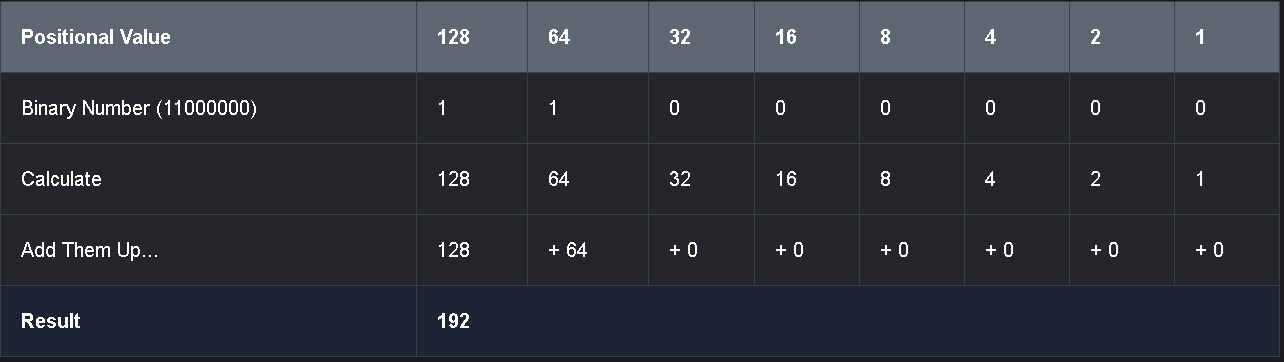
\includegraphics[width=\textwidth]{13.png}
    \caption{Convert Binary to Decimal}
    \label{fig:cap1}
\end{figure}

\begin{enumerate}
    \item Binary to Decimal Conversion:\\
    \begin{itemize}
        \item An IPv4 address is a 32-bit binary number divided into four 8-bit octets.\\
        \item To convert binary to decimal:\\
        \begin{itemize}
            \item Break the binary address into four actets.\\
            \item Use positional notion (powers of 2) to calculate the decimal values of each octet.\\
            \item Example: Binary $11000000.10101000.00001011.00001010$ converts to $192.168.11.10$.\\
        \end{itemize}
    \end{itemize}
    \item Decimal to binary Conversion:\\
    \begin{itemize}
        \item To convert decimal to binary:\\
        \begin{itemize}
            \item Start with the highest positional values (128) and work down to the lowest(1).
            \item For each bit, ask: Is the decimal number mayor to the positional values?\\
            \begin{itemize}
                \item If yes, write 1 and subtract the positional values from the decimal number.\\
                \item if no, write 0.\\
            \end{itemize}
        \end{itemize}
        \item Exampla: Decimal 192 converts to binary 11000000.\\
    \end{itemize}
\end{enumerate}

\title{Example:}\\
\begin{itemize}
    \item Start with teh decimal number (e.g., 192).\\
    \item Compare it to positional values (128, 64, 32, 16, 8, 4, 2, 1):\\
    \begin{itemize}
        \item Is 192 larger than 128? yes, write 1, subtract 128, remaining: 64.\\
        \item Is 64 larger than 64 yes write 1, subtract 64, remaining: 0\\
        \item Fill the rest with 0.\\
    \end{itemize}
\end{itemize}

\title{Hexadecimal Number System}\\
Think of hexadecimal as a shorthand for binary. Just as you might abbreviate a long word to save time, Hexadecimal abbreviates long binary strings into shorter, more manageable forms.\\
\begin{enumerate}
    \item Hexadecimal Basics:\\
    \begin{itemize}
        \item Hexadecimal is a base-16 numbering system.\\
        \item It uses digits 0-9 and letters A-F to represent values.\\
        \item Examples: Binary 0000 = Decimal 0 = Hexadecimal 0; Binary 1111 = Decimal 15  = Hexadecimal F.\\
    \end{itemize}
    \item Why Hexadecimal?:\\
    \begin{itemize}
        \item Hexadecimal is more compact than binary. For example, 4 binary bits (1111) can be represented as a single hexadecimal digit (F).\\
        \item It is widely used in networking for IPv6 addresses and Ethernet MAC a addresses.\\
    \end{itemize}
    \item IPv6 Addresses:\\
    \begin{itemize}
        \item IPv6 addresses are 128 bits long, divided into 32 hexadecimal digits (each repesenting 4 bits).\\
        \item The preferred format for IPv6 addresses is x:x:x:x:x:x:x:x, Where each x is a hextet (16 bits or 4 hexadecimal digits).\\
    \end{itemize}
    \item Hextets:\\
    \begin{itemize}
        \item A hextet is a unofficial term for a 16-bit segment of an IPv6 address (4 hexadecimal digits).\\
        \item Each hextet represents a portion of the 128-bit IPv6 address.\\
    \end{itemize}
    \item Case Insensitivity:\\
    \begin{itemize}
        \item can be written in uppercase or lowercase.\\
    \end{itemize}
\end{enumerate}

\begin{figure}[h!]
    \centering
    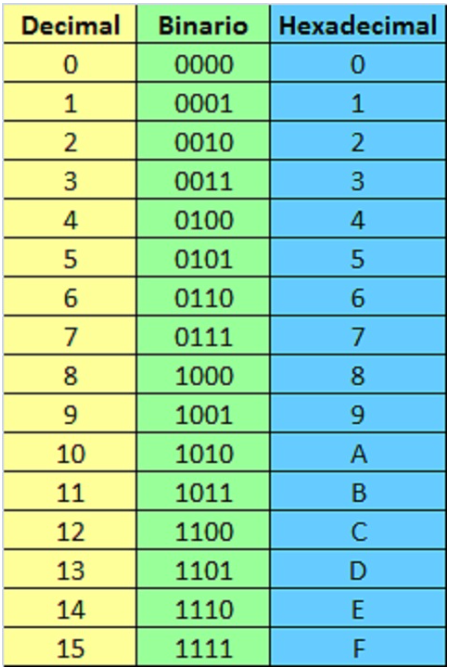
\includegraphics[width=0.4\textwidth]{14.png}
    \caption{S. Hexadecimal}
    \label{fig:cap1}
\end{figure}

\title{Decimal and Hexadecimal Conversion}
\begin{enumerate}
    \item Convert the decimal number into an 8-bit binary string.\\
    \item Splilt the binary string into groups of four, starting from the right.\\
    \item Convert each group into its hexadecimal equivalent.\\
\end{enumerate}

% Ejemplo del cuadro con información en grises y blancos
\begin{tcolorbox}[colframe=gray!80, colback=gray!20, coltitle=black, title= Example: ]
168 in banary = 10101000; split: 1010 (A) and 1000(8)8; 168 in hexadecimal = A8
A8
\end{tcolorbox}

\newpage
\title{Hexadecimal to Decimal Conversion}\\
\begin{enumerate}
    \item Convert each hex digit into a 4-bit binary strng.\\
    \item Combine into an 8-bit binary grouping.\\
    \item Convert the binary number into decimal.\\
\end{enumerate}

% Ejemplo del cuadro con información en grises y blancos
\begin{tcolorbox}[colframe=gray!80, colback=gray!20, coltitle=black, title= Example: ]
D2 in Hex = 1101 (D) 0010 (2); combined: 11010010 in decimal = 210
\end{tcolorbox}

\newpage
\section{Purpose of the Data Link Layer}
The Dta Link (Layer 2) of the OSI model is responsible for preparing data to be transmitted over the physical network, It plays a critical role in enabling communication between network devices at the hardware level (i.e., between Network Interface Cards (NICs)) and is responsible for the following tasks:\\

\title{Key Responsibilities:}\\
\begin{enumerate}
    \item Enable upper layers to access the media: Provides a standard method for accessig the network media (Ethernet, Wi-Fi, etc), making the upper layers unaware of the specific media type being used.\\
    \item Encapsulation Layer 3 packets: The Data Link Layer accepts Layer 3 packets (like IPv4 or IPv6) and encapsulates them into frames suitable for transmission over the network medium.\\
    \item Data transfer control: It controls how  data is placed and received on the physical media.\\
    \item Frame exchanges: It exchanges frames between nodes accross the network.\\
    \item Error detection: It performs error detection and rejects corrupted frames.
    \item Error detection: It performs error detection and rejects any corrupted frames.\\
\end{enumerate}

\begin{figure}[h!]
    \centering
    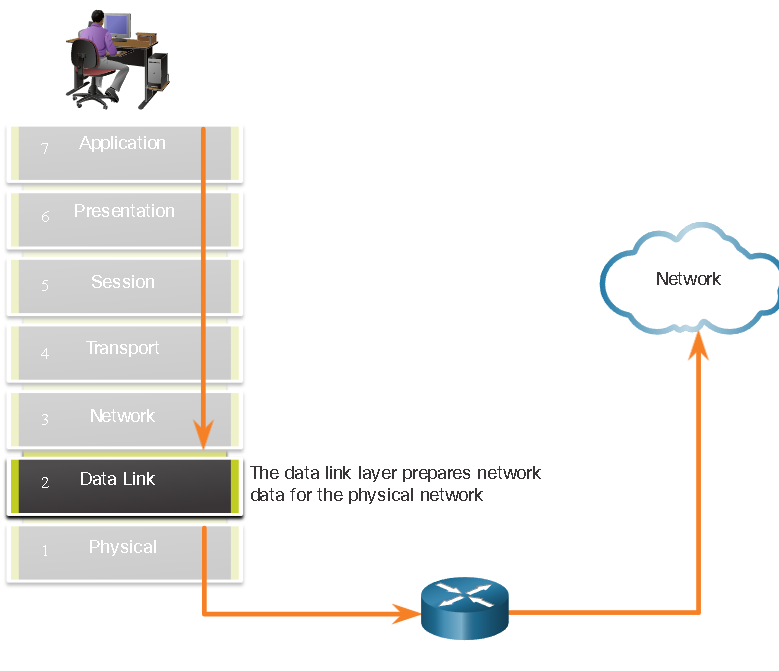
\includegraphics[width=0.65\textwidth]{15.png}
    \caption{S. Data Link}
    \label{fig:cap1}
\end{figure}

\begin{figure}[h!]
    \centering
    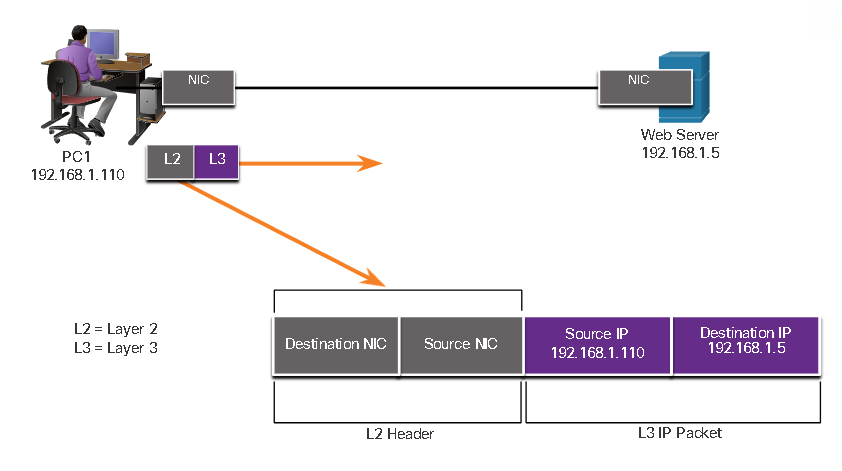
\includegraphics[width=\textwidth]{16.png}
    \caption{Example of Data Link Layer Adding Ethernet Destination and Source Information to a Layer 3 Packet}
    \label{fig:cap1}
\end{figure}

\title{IEEE 802 LAN/MAN Data Link Sublayers:}
IEEE 802 defines standards for various LAN/MAN technologies like Ethernet (802.3), Wi-Fi (802.11), and others. The Data Layer is divided into two main sublayers:\\

\begin{enumerate}
    \item Logical Link Control (LLC):\\
    \begin{itemize}
        \item This sublayer communicates between the upper-layer protocols and the lower hardware layers.\\
        \item It adds control information to the data, enabling multiple Layer 3 protocols (like IPv4 and IPv6) to use the same network interface.\\
    \end{itemize}
    \item Media Access Control (MAC):\\
    \begin{itemize}
        \item The MAC sublayer controls the hardware resposnsible for data encapsulation and access to the network medium.\\
        \item It defines the addressing system and error detection method (like CRC checksums).\\
        \item It also defines how devices devices gain access to a shared medium, especially in cases like Ethernet or Wi-Fi.\\
    \end{itemize}
\end{enumerate}

\begin{figure}[h!]
    \centering
    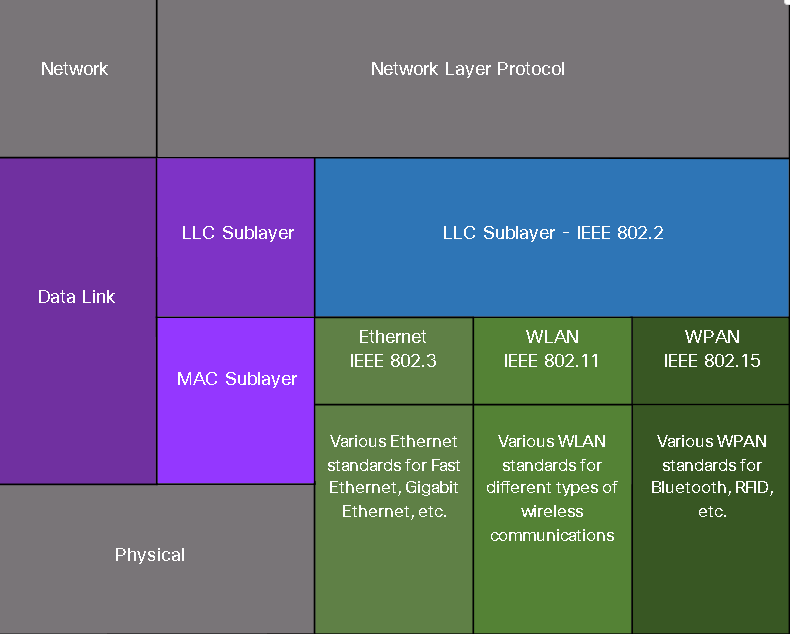
\includegraphics[width=0.75\textwidth]{17.png}
    \caption{Data Link Sublayers}
    \label{fig:cap1}
\end{figure}

\title{Access to Media:}\\
The Data Link Layer a crucial role in allowing devices to share the communication medium. Manages how data are accessed, transferred, and synchronized between devices in a network. For example:\\

\begin{itemize}
    \item In Ethernet LANs, multiples devices may be competing for access to the network medium, and the MAC sublayer resolves this contention.\\
    \item In serial connections, such as between two routers, direct communication may take place without contention, requiring simpler media access methods.\\
\end{itemize}

\title{Router Operation:}\\
Routers use the Data Link Layer services when forwarding data between different segments of a network. A router does the following when processing data:\\

\begin{enumerate}
    \item Accepts a frame from a medium.\\
    \item De-encapsulates the frame to retrieve the Layer 3 packet (Ip packet).\\
    \item Re-encapsulates teh packet into a new frame appropriate for the next network segment (with appropriate Layer 2 addressing and error detection).\\
    \item Forwards the new frame to the appropriate medium for transmission.
\end{enumerate}

\begin{figure}[h!]
    \centering
    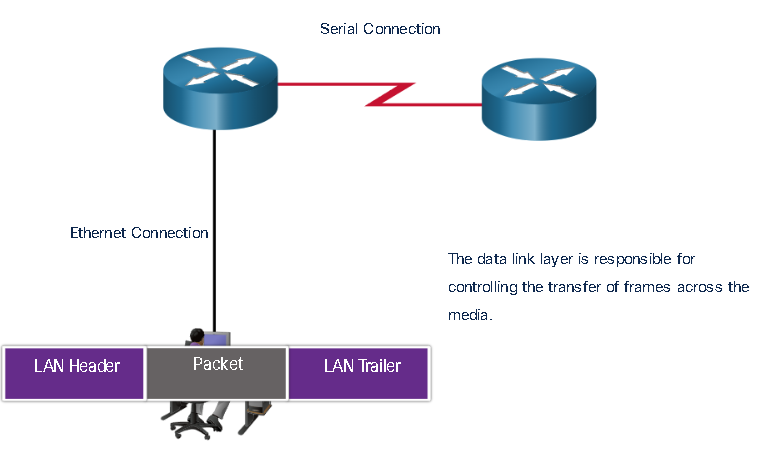
\includegraphics[width=0.65\textwidth]{18.png}
    \caption{Access to Media}
    \label{fig:cap1}
\end{figure}

\begin{figure}[h!]
    \centering
    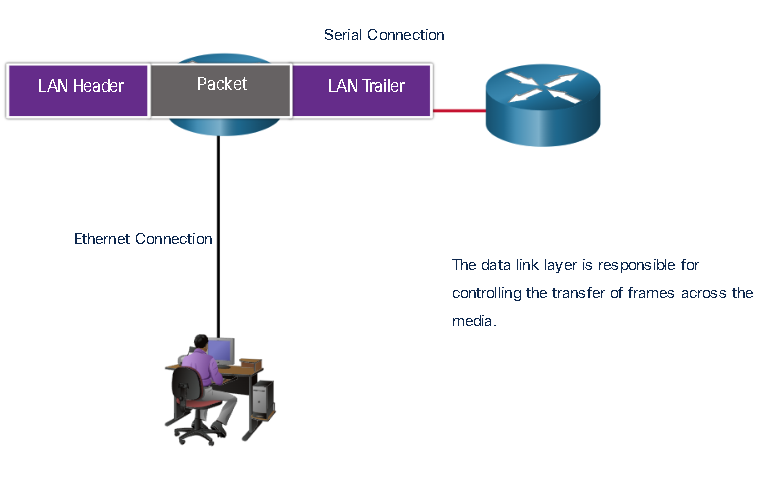
\includegraphics[width=0.65\textwidth]{19.png}
    \caption{Access to Media}
    \label{fig:cap1}
\end{figure}

\begin{figure}[h!]
    \centering
    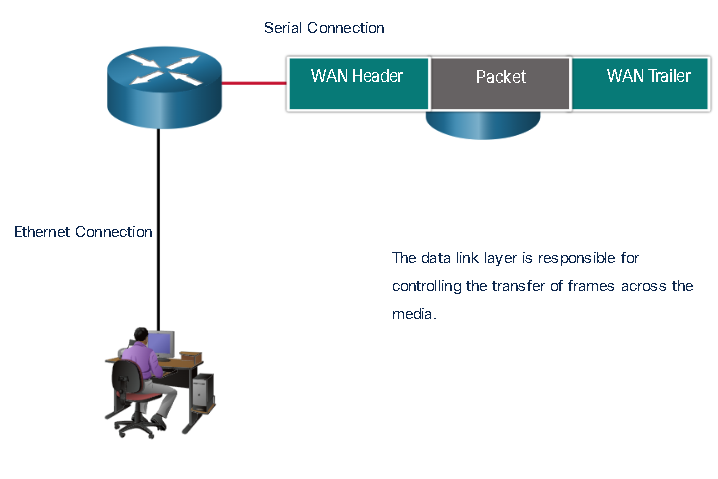
\includegraphics[width=0.65\textwidth]{20.png}
    \caption{Access to Media}
    \label{fig:cap1}
\end{figure}

The Data Link Layer thus ensures smooth communication between devices within a network by managing how data is framed, addressed, and transferred across different media types.\\

\subsection{Topologies}\\
Topologies are essential for understanding how networks function at the data link laye. These topologies describe how devices are connected (physically) and how data is transferred (logically) across a network.\\

\title{Key Points}\\
\begin{enumerate}
    \item Physical Topology: is like the actual roads and intersection (how things are physically laid out).\\
    \begin{itemize}
        \item Describes the actual layout of devices and connections in a network.\\
        \item Includes details like devices locations,  types of cables and hardware setups.\\
        \item Common physical topologies include:\\
        \begin{itemize}
            \item Point-to-point: A direct connection between two nodes.\\
    \begin{figure}[h!]
    \centering
    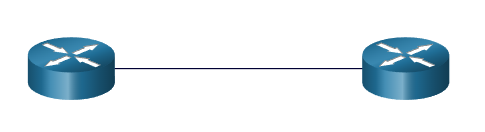
\includegraphics[width=0.2\textwidth]{23.png}
    \caption{Point-to-point}
    \label{fig:cap1}
    \end{figure}
            \item Start: Devices connect to a central hub or switch. Is like a roundabout where all roads lead to a central hub.\\
            \item Extended Start:  Multiples star topologies interconnected via switches.\\
            \item Bus: Devices are connected along a single shared cable (legacy Ethernet). Is like a single highway where all cars share the same lane.\\
            \item Ring: Devices form a closed loop where each node connects to its neighbors (e.g., Token Ring).\\
        \end{itemize}
    \end{itemize}

    \begin{figure}[h!]
    \centering
    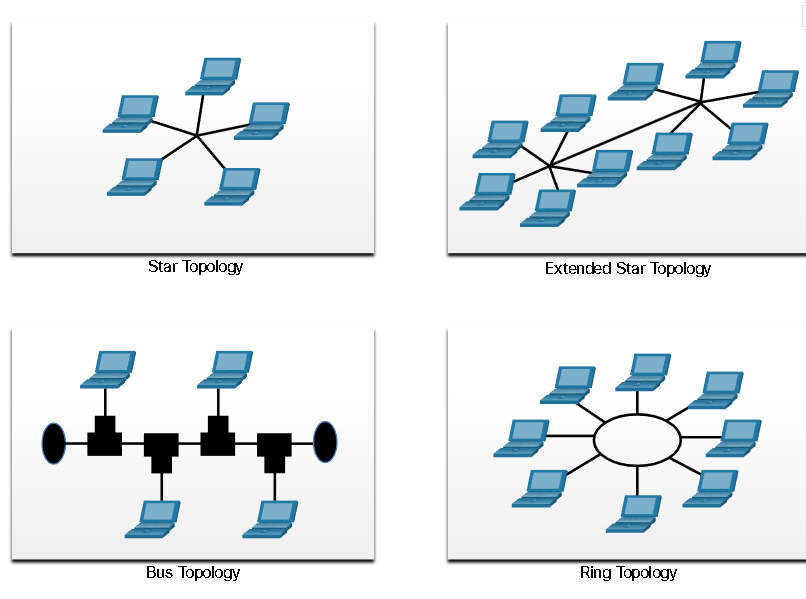
\includegraphics[width=0.4\textwidth]{28.png}
    \caption{Physical Topology}
    \label{fig:cap1}
    \end{figure}
    
    \begin{figure}[h!]
    \centering
    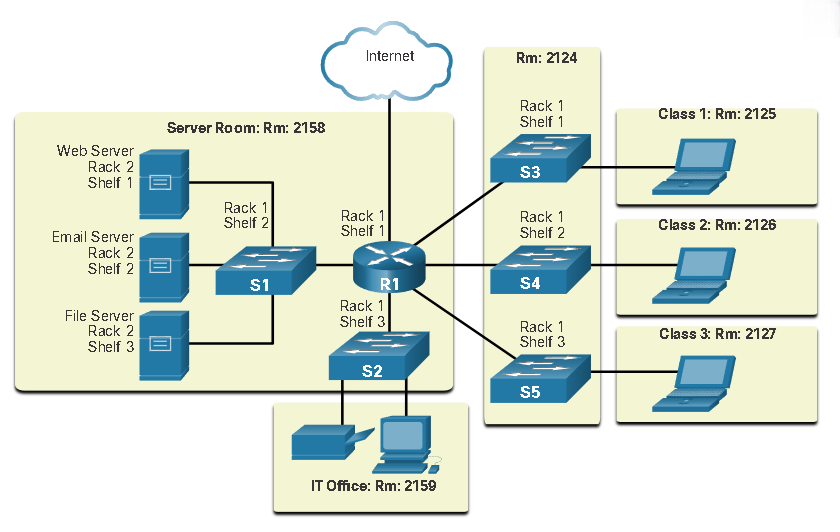
\includegraphics[width=0.6\textwidth]{21.png}
    \caption{Physical Topology}
    \label{fig:cap1}
    \end{figure}
    
    \item Logical Topology:Is like the traffic flow rules(how cars move and interact on those roads).\\
    \begin{itemize}
        \item Refers to how data flows between devices, regardless of the physical layout.\\
        \item Determines how frames are transferred and how media access is controlled.\\
        \item Examples include point-to-point logical connections, even if the physical topology involves multiple intermediary devices.\\
    \end{itemize}

    \begin{figure}[h!]
    \centering
    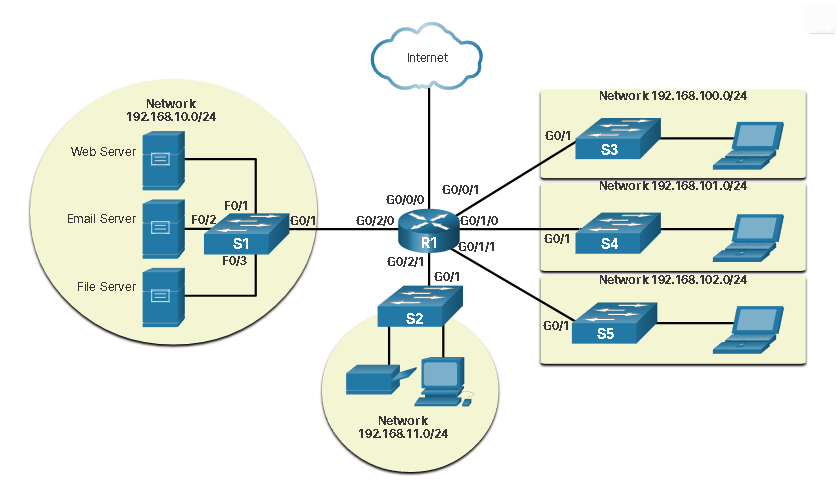
\includegraphics[width=0.6\textwidth]{22.png}
    \caption{Logical Topology}
    \label{fig:cap1}
    \end{figure}

    \item Wan Topologies:\\
    \begin{itemize}
        \item WANs often use specific physical topologies:\\
        \begin{itemize}
            \item Point-to-point: Simplest topology with a direct link between two endpoints.\\

    \begin{figure}[h!]
    \centering
    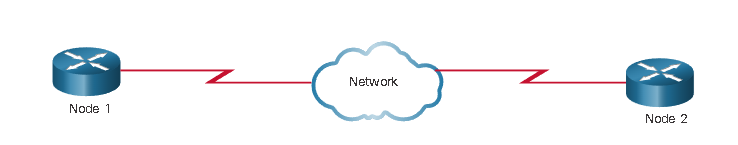
\includegraphics[width=0.5\textwidth]{26.png}
    \caption{Point-to-point}
    \label{fig:cap1}
    \end{figure}
\newpage
            \item Hub-and-spoke: A central site connects to multiples branch sites via point-to point links; branches cannot communicate directly.\\
    \begin{figure}[h!]
    \centering
    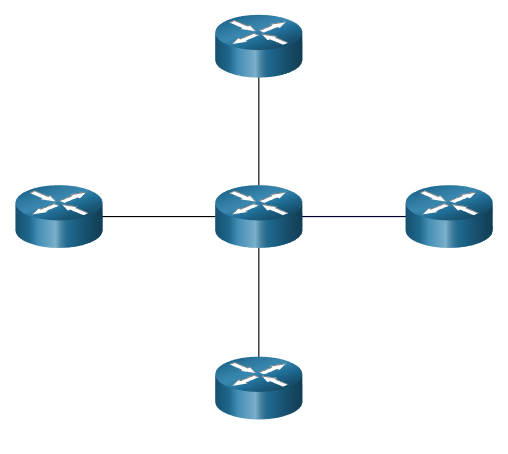
\includegraphics[width=0.25\textwidth]{24.png}
    \caption{Hub-and-spoke}
    \label{fig:cap1}
    \end{figure}
            \item Mesh: Every device connects to every other device, providing high availability but at higher cost. Is like a city grid where every intersection connects to every other intersection.\\
    \begin{figure}[h!]
    \centering
    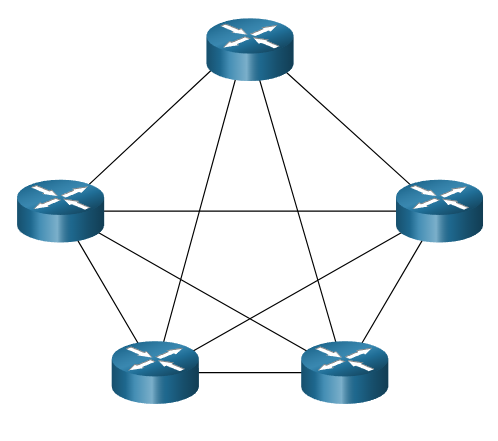
\includegraphics[width=0.25\textwidth]{25.png}
    \caption{Mesh}
    \label{fig:cap1}
    \end{figure}
            \item Hybrid: Combines elements of different topologies (e.g., partial mesh).\\
        \end{itemize}
    \end{itemize}
    \item Duplex Communication:\\
    \begin{itemize}
        \item Half-Duplex: Devices can send or receive data, but not simultaneously (e.g., legacy Ethernet hubs, WLANs). Is like a one-lane bridge where cars take turns crossing.\\

    \begin{figure}[h!]
    \centering
    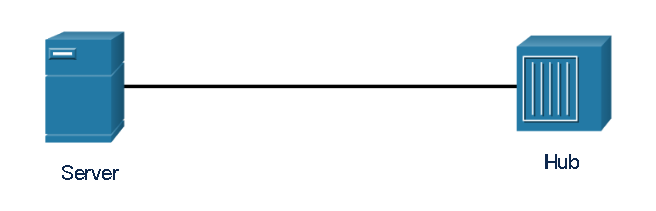
\includegraphics[width=0.41\textwidth]{29.png}
    \caption{Half-Duplex}
    \label{fig:cap1}
    \end{figure}
        
        \item Full-duplex:Devices can send receive data simultaneously (e.g., modern Ethernet switches). Is like a two-lane highway where cars can travel in both directions simultaneously.\\

    \begin{figure}[h!]
    \centering
    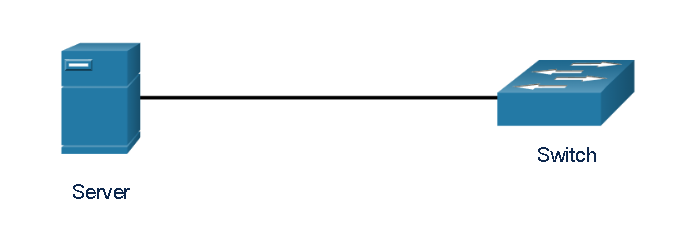
\includegraphics[width=0.4\textwidth]{30.png}
    \caption{Full-duplex}
    \label{fig:cap1}
    \end{figure}
        
        \item Mismatched duplex settings between devices cause inefficiencies and latency.\\
    \end{itemize}
    \item Access Control Methods:Selecting appropriate access control methods prevents data collisions and improves performance.\\
    \begin{itemize}
        \item Multi access networks (e.g., Ethernet LANs, WLANs) require rules to manage how devices share the medium.\\
        \begin{itemize}
            \item Contention-based access:\\
            \begin{itemize}
                \item Devices compete for the medium (e.g., CSMA/CD for Ethernet, CSMA/CA for WLANs).\\
                \item Only one device can transmit at a time.\\
            \end{itemize}

    \begin{figure}[h!]
    \centering
    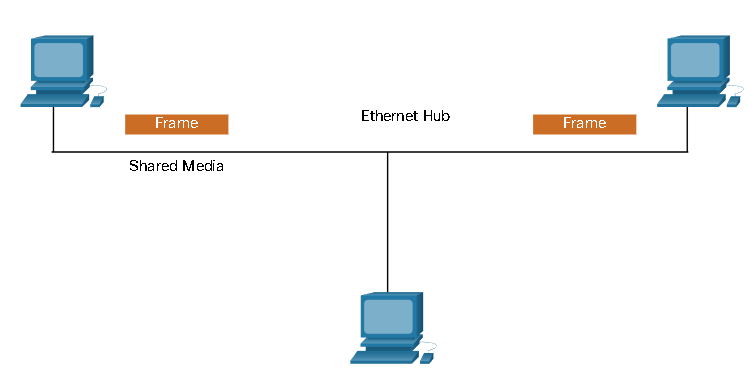
\includegraphics[width=0.4\textwidth]{31.png}
    \caption{Full-duplex}
    \label{fig:cap1}
    \end{figure}
            
            \item Controlled access:\\
            \begin{itemize}
                \item Each device gets a turn to use the medium, ensuring no collisions but reducing efficiency.\\
    \begin{figure}[h!]
    \centering
    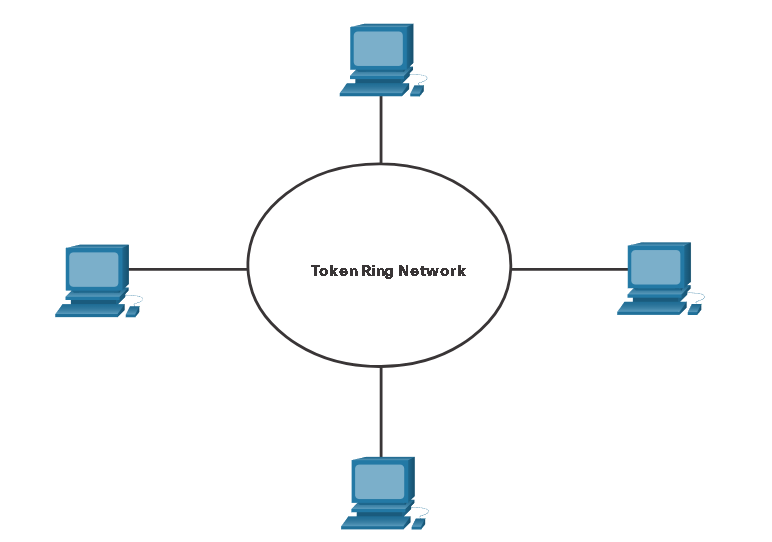
\includegraphics[width=0.4\textwidth]{32.png}
    \caption{Full-duplex}
    \label{fig:cap1}
    \end{figure}
                
            \end{itemize}
        \end{itemize}
    \end{itemize}
\end{enumerate}

\newpage
\subsection{Data Link Frame}
It focuses on how frames are structured, the fields they contain, and the protocols used to manage communication at this layer. Think of the data link layer as the postal service for your network.\\

\begin{figure}[h!]
\centering
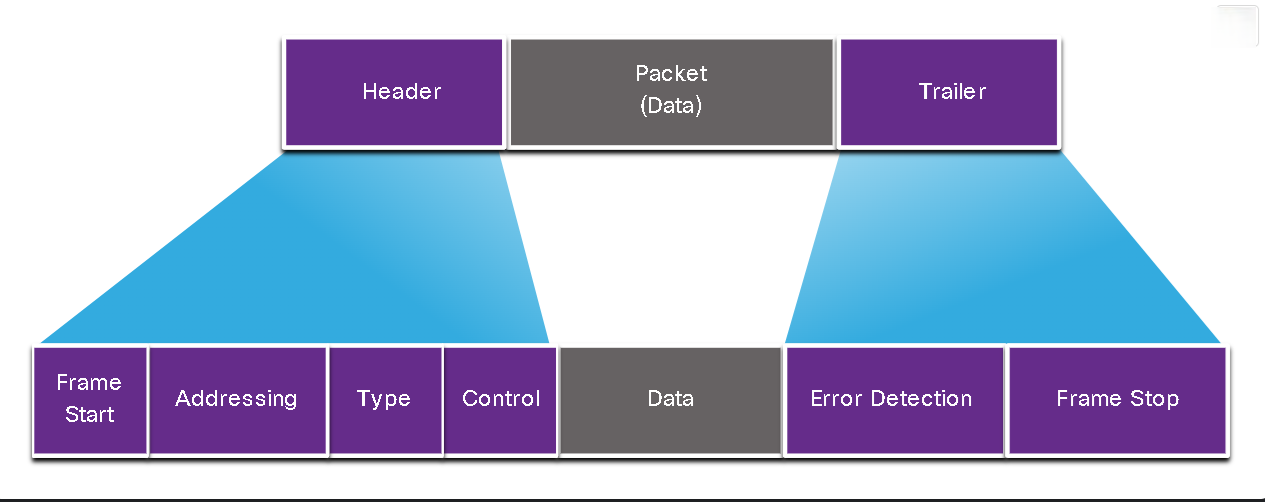
\includegraphics[width=0.7\textwidth]{33.png}
\caption{Full-duplex}
\label{fig:cap1}
\end{figure}

\title{Key Points}
\begin{enumerate}
    \item Frame Structure:\\
    \begin{itemize}
        \item A frame consists of three main parts: is like an envelope that wraps your letter(data).\\
        \begin{itemize}
            \item Header: Contains control information such as source and destination addresses, type of protocol (e.g., IPv4 or IPv6), and quality of service (QoS) settings.(the "to" and "from" addresses).\\
            \item Data: Encapsulates the payload, which includes the packet from the network layer(Layer 3). Is like the letter.\\
            \item Trailer: Includes error detection mechanism like the frame check Sequence (FCS)  to ensure data integrity during transmission. A checksum to ensure the letter wasn't damaged in transit\\
        \end{itemize}
        \item The structure of the frame varies depending on the protocol and media type.\\
    \end{itemize}
    \item Error Detection: If the letter gets damaged (e.g., torn or smudged), the recipient can tell using the checksum and request a resend.\\
    \begin{itemize}
        \item The trailer contains a Cyclic Redundancy Check (CRC) value, which is a mathematical summary of the frame's contents. This allows the receiving node to detect errors caused by interference, distortion, or loss during transmission.\\
    \end{itemize}
    \item Layer 2 (Physical) Addressing:\\
    \begin{itemize}
        \item The data link layer uses physical addresses (e.g., MAC addresses) to identify devices within the same local network.\\
        \item These addresses are flat (non-hierarchical) and only meaningful within the local network segment.\\
        \item When data moves between networks, an intermediary device like a router in a new frame for the next hop.\\
    \end{itemize}
    \item Protocols for Different Network Types:\\
    \begin{itemize}
        \item LANs typically use protocols like Ethernet (wired) and IEEE 802.11 (WLAN) (wireless), designed for multi access environments with high bandwidth.\\
        \item WANs traditionally use protocols like PPP, HDLC, Frame Relay, and ATM, optimized for lower bandwidth and long-distance communication. However, Ethernet is increasingly replacing these older WAN protocols.\\
    \end{itemize}
    \item Encapsulation Process:\\
    \begin{itemize}
        \item Encapsulation Process:\\
        \begin{itemize}
            \item Host-to-router: The host adds its MAC address as the source and the router's MAC address as teh destination.\\

\begin{figure}[h!]
\centering
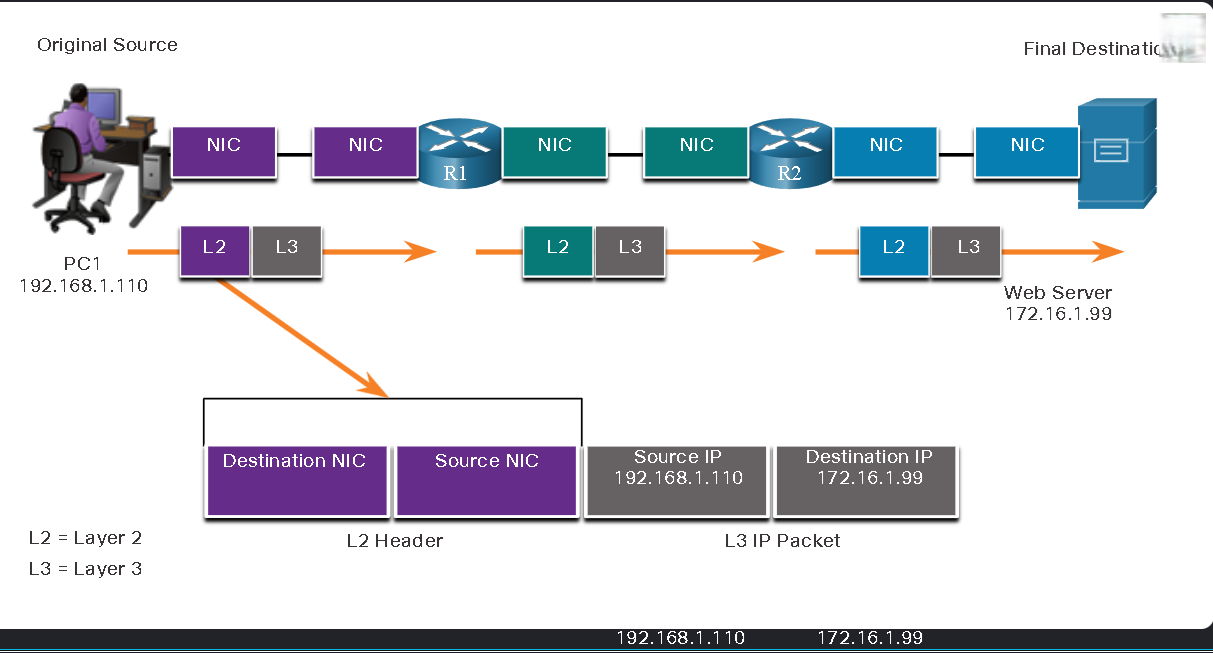
\includegraphics[width=0.75\textwidth]{34.png}
\caption{Host-to-router}
\label{fig:cap1}
\end{figure}

            
            \item Router-to-router: Each router replaces the frame header with its own MAC address as the source and the next-hop router's MAC address as the destination.\\

\begin{figure}[h!]
\centering
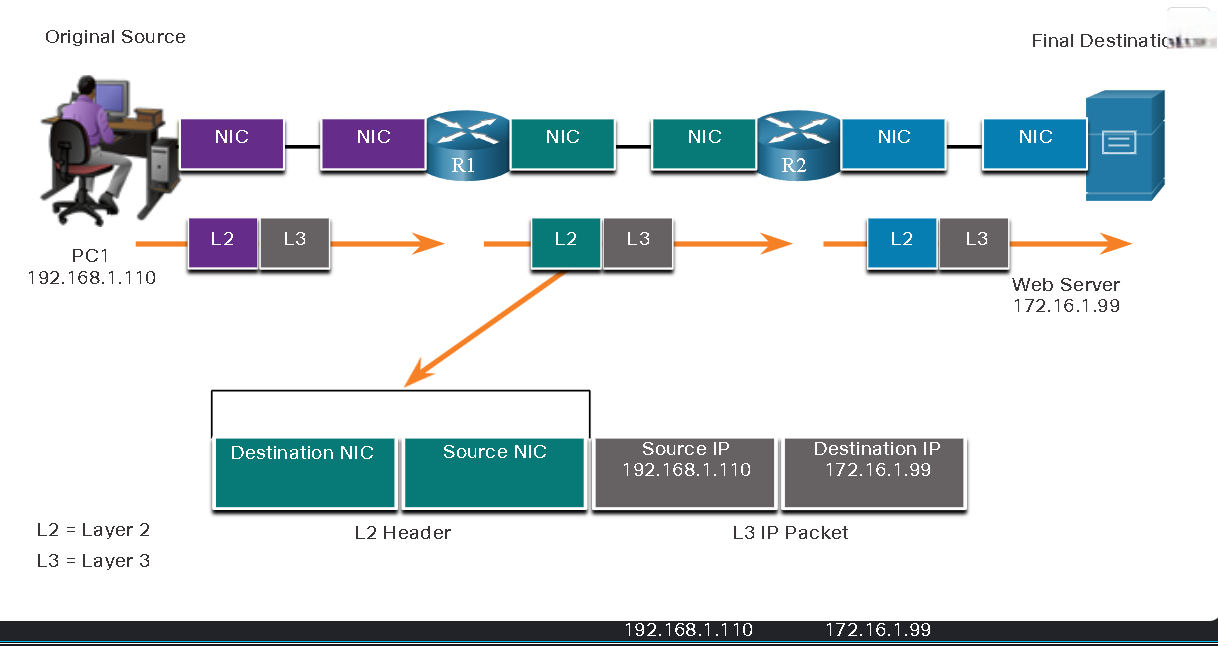
\includegraphics[width=0.75\textwidth]{35.png}
\caption{Router-to-router}
\label{fig:cap1}
\end{figure}

            
            \item Router-to-host: The final router encapsulates the packet with its MAC address as the source and the destination host's MAC address as the destination.\\

\begin{figure}[h!]
\centering
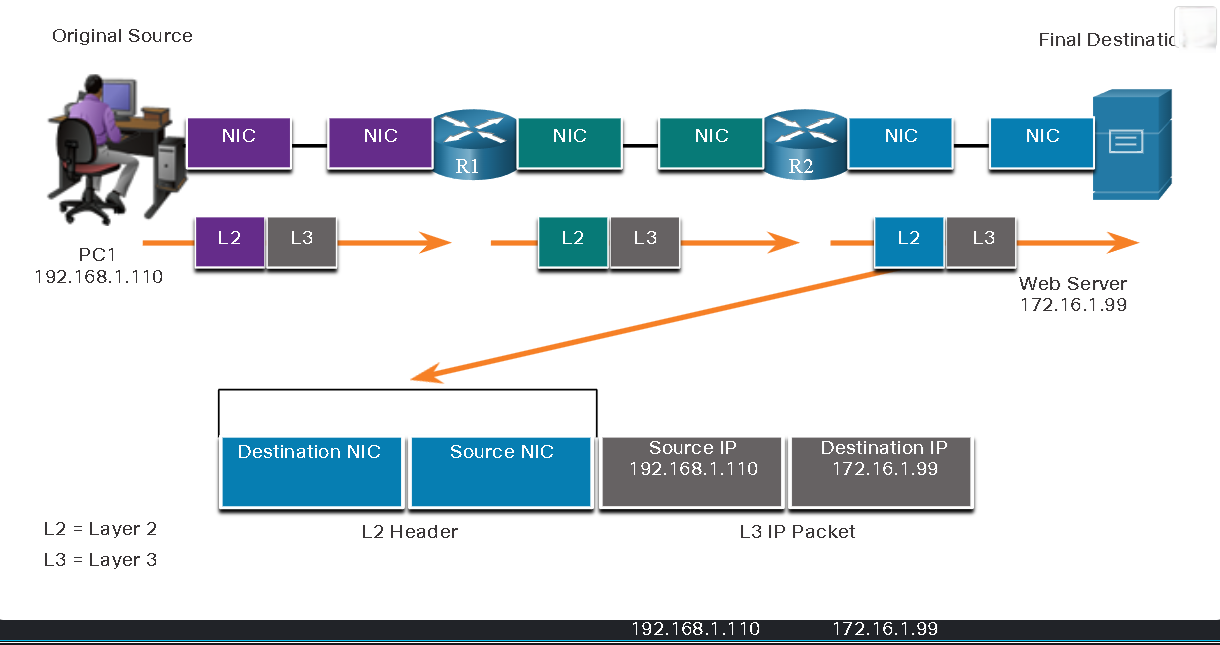
\includegraphics[width=0.75\textwidth]{36.png}
\caption{Router-to-host}
\label{fig:cap1}
\end{figure}

            
        \end{itemize}
    \end{itemize}
    \newpage
    \item Differences Between LANs and WANs:\\
    \begin{itemize}
        \item LANs:\\
        \begin{itemize}
            \item High bandwidth, suitable for dense user environments like campuses or buildings.\\
            \item Cost-effective due to smaller geographic scope.\\
        \end{itemize}
        \item WANs:\\
        \begin{itemize}
            \item Lower bandwidth due to the cost of long-distance links.\\
            \item Used specialized protocols for point-to-point, hub-and-spoke, or mesh topologies.\\
        \end{itemize}
    \end{itemize}
    \item Examples of Data Link Layer Protocols:\\
    \begin{itemize}
        \item LAN Protocols: Ethernet, IEEE 802.11 (Wi-Fi).\\
        \item WAN Prtocols: PPP, HDLC, Frame Relay, ATM, x.25.\\
    \end{itemize}
\end{enumerate}

\newpage
\section{ Ethernet Switching}
Its operation in the OSI model, and the structure of its frames. Ethernet operates at both the data link layer (Layer 2) and the physical layer (Layer 1 ), Supporting various bandwidth (e.g., 10 Mbps to 100 Gbps). It uses two sublayers in the data link layer. The logical link control LLC and the Media Access Control (MAC). Think of an Ethernet frame as a packge being sent through the mail. \\
\title{Key Points:}
\begin{enumerate}
    \item Ethernet Overview:\\
    \begin{itemize}
        \item Ethernet is a family of networking technologies defined by IEEE standards (802.3 for wired Ethernet, 802.11 for wireless).\\
        \item It supports multiple bandwidths, ranging from 10 Mbps to Gbps.\\
        \item Ethernet Operation in both the data link layer (framing, addressing, error detection) and the physical layer (media specification like twisted pair, fiber, etc.).\\
    \end{itemize}
    \item Data Link Sub-layers:\\
    \begin{itemize}
        \item LLC Sublayer (IEEE 802.2):\\
        \begin{itemize}
            \item Communicates between upper-layer protocols (e.g., IPv4, IPv6) and hardware.\\
            \item Adds information to identify the network layer protocols being used.\\
        \end{itemize}
        \item MAC Sublayer (IEEE 802.3):\\
        \begin{itemize}
            \item Implemented in hardware (e.g., NICs).\\
            \item Responsible for data encapsulation, addressing, and media access control.\\
            \item Include mechanism like CSMA/CD for half-duplex communication (legacy Ethernet) and supports full-duplex communication with modern switches.\\
        \end{itemize}
    \end{itemize}
    \item Ethernet Frame Fields:The Ethernet frame has several fields, each serving a specific purpose:\\
    \begin{itemize}
        \item Preamble (7 bytes) + Start Frame Delimiter (SFD)(1 byte):\\
        \begin{itemize}
            \item Used for synchronization between sender and receiver.\\
        \end{itemize}
        \item Destination MAC Address (6 bytes):\\
        \begin{itemize}
            \item Identifies the intended recipient of the frame (unicast, multicast, or broadcast).\\
        \end{itemize}
        \item Source MAC Address (6 bytes):\\
        \begin{itemize}
            \item Identifies the sender's  NIC or  interface.\\
        \end{itemize}
        \item Type/Length Field (2 bytes):\\
        \begin{itemize}
            \item Specifies the upper-layer protocol encapsulated in the frame (e.g., IPv4, IPv6, ARP).
        \end{itemize}
        \item Data Field (46-1500 bytes):\\
        \begin{itemize}
            \item Contains the payload from higher layer (e.g., an IPv4 packet).\\
            \item If the payload is smaller than 46 bytes, padding is added to meet the minimum frame size.\\
        \end{itemize}
        \item Frame Check Sequence (FCS) (4 bytes):\\ 
        \begin{itemize}
            \item Used for error detection via Cyclic Redundancy Chec (CRC).\\
            \item The sender Calculates a CRC value and includes it in the FCS field the receiver recalculates the CRC to check for error.\\
        \end{itemize}
    \end{itemize}
    \item Frame Size:\\
    \begin{itemize}
        \item Minimum Frame Size: 64 bytes (including all fields except the preamble).\\
        \item Maximum Frame Size: 1518 bytes (standard) or larger for jumbo frames (common in Fast Ethernet and Gigabit Ethernet).\\
        \item Frames larger than 64 bytes are called collision fragments or runt frames and are discarded.\\
        \item Frames larger than 1500 bytes are considered jumbo frames and may require special support.
    \end{itemize}
    \item Access Methods:\\
    \begin{itemize}
        \item Legacy Ethernet (half-duplex): Used CSMA/CD to manage shared media and detect collisions.\\
        \item Modern Ethjernet (full-duplex): Switches eliminates the need for CSMA/CD by allowing simultaneous.\\
    \end{itemize}
\end{enumerate}

\title{Simplified Explanation:}\\
Think of an Ethernet frame as a package being sent through the mail.\\
\begin{itemize}
    \item The preamble is like ringing the doorbell to get the recipient's attention.\\
    \item The Destination and source MAC addresses are like the "to" and "from" labels on the package.\\
    \item The Type/length field tells the recipient what's inside the package (e.g., a letter, a gift).\\
    \item The Data field contains the actual contens fo the package.\\
    \item The FCS is like a seal that ensures the package wasn't  demaged during delivery.
\end{itemize}

If the package is too small or too large, it's rejected because it doesn't meet the standard requirements.\\

\end{document}